\documentclass[11pt]{article}

% --- Geometry & typography ---
\usepackage[margin=1in]{geometry}
\usepackage{microtype}
\usepackage{lmodern}
\usepackage[T1]{fontenc}

% --- Math & symbols ---
\usepackage{amsmath,amssymb,amsthm}

% --- Graphics ---
\usepackage{graphicx}
\graphicspath{{figs/}}

% --- Tables ---
\usepackage{booktabs}
\usepackage{array}
\usepackage{multirow}
\usepackage{makecell}

% --- Code listings ---
\usepackage{listings}
\usepackage{xcolor}
\definecolor{codebg}{rgb}{0.97,0.97,0.97}
\definecolor{codekw}{rgb}{0.10,0.10,0.55}
\definecolor{codestr}{rgb}{0.55,0.10,0.10}
\definecolor{codecmt}{rgb}{0.40,0.40,0.40}
\lstset{
  backgroundcolor=\color{codebg},
  basicstyle=\footnotesize\ttfamily,
  keywordstyle=\color{codekw}\bfseries,
  stringstyle=\color{codestr},
  commentstyle=\color{codecmt}\itshape,
  showstringspaces=false,
  breaklines=true,
  frame=single,
  rulecolor=\color{black!20},
  numbers=none,
  captionpos=b,
  language=Python,
}

% --- Hyperlinks ---
\usepackage[colorlinks=true,linkcolor=blue!50!black,citecolor=blue!50!black,urlcolor=blue!50!black]{hyperref}

% --- Caption styling ---
\usepackage{caption}
\captionsetup{font=small,labelfont=bf,labelsep=period,skip=4pt}

% --- Spacing ---
\setlength{\parskip}{0.5em}
\setlength{\parindent}{0pt}

% --- Custom commands ---
\newcommand{\skyd}{\textsc{SkyDiscover}}
\newcommand{\adaev}{AdaEvolve}
\newcommand{\bcontroller}{\texttt{BatchedAdaEvolveController}}
\newcommand{\todo}[1]{\textcolor{red}{\textbf{TODO:} #1}}

\title{
  \vspace{-1.5em}
  \large \textbf{Cache-Aware Parallel \adaev{}: A Systems Study of GPU-Efficient LLM-Guided Evolutionary Search}\\[0.3em]
  \normalsize Project report --- computer systems exploration on top of \skyd{}'s evolutionary search algorithm
}


\date{April 30, 2026}

% =============================================================================
\begin{document}
\maketitle

% =============================================================================
\begin{abstract}
\noindent
\skyd{} is an LLM-guided evolutionary code-discovery framework whose
flagship search algorithm, \adaev{}, samples a parent program, asks an
LLM to mutate it, evaluates the child, and iterates. Each iteration
today issues exactly one LLM call against vLLM with prefix caching;
on real workloads (\skyd{}'s prior \texttt{KV\_CACHING\_REPORT.md}
measured \emph{17.3\,\%} effective hit rate) most of the per-iteration
prompt churns and the engine cache is largely wasted.

This report presents a stack of seven systems-level optimizations on
top of \adaev{}, ordered by implementation cost from a one-week
controller change to a multi-month vLLM internals modification:
\textbf{(1)}~$K$-batched candidates per iteration sharing a single prompt;
\textbf{(2)}~adaptive $K$ keyed off \adaev{}'s exploration intensity
signal; \textbf{(3)}~speculative iteration pipelining with
GPU-pressure-aware gating; \textbf{(4)}~multi-problem orchestration on
a shared vLLM endpoint; \textbf{(5)}~AdaEvolve-aware priority eviction
overriding vLLM's LRU; \textbf{(6)}~persistent KV across runs
snapshotting the system prefix; and \textbf{(7)}~diff-aware
cross-iteration KV reuse with RoPE re-application.

Each optimization is measured in isolation and stacked, on a real
vLLM endpoint serving Qwen3-4B-Instruct-2507 on an H100 where
possible, and on a chained-SHA-256 / 16-token-block faithful
simulator for the items requiring vLLM internals modification.
On \texttt{circle\_packing} and \texttt{signal\_processing}, two
file-evaluator benchmarks from \skyd{}'s math suite, the headline
numbers are: \textbf{cache hit rate climbs from 18.4\,\% to 94.2\,\%},
\textbf{per-call wall-time speedup of 9.8$\times$} at the canonical
2-bench cohort and \textbf{10.6$\times$} at single-problem $N\!=\!8$,
and \textbf{best score on \texttt{circle\_packing} reaches 0.816} in 16
iterations (seed 0.364, AlphaEvolve target 1.000) confirming the
optimizations preserve search quality. We also report \textbf{47--52\,\%
additional GPU prefill reduction} from diff-aware KV reuse in
simulation, and a \textbf{71\,\% reduction} in a stable tenant's GPU
prefill cost from priority eviction under multi-tenant pressure.

The paper closes with three methodological corrections that shifted
measured effects by large factors and that we believe generalize to
anyone benchmarking LLM-guided search systems.
\end{abstract}

\tableofcontents
\vspace{1em}

% =============================================================================
\section{Introduction}
\label{sec:intro}

\subsection{Problem context}

\skyd{}~\cite{skydiscover2026} is an open framework for LLM-guided
discovery: it provides a database of programs, an evolutionary
controller, an evaluator interface, and integrations with multiple
LLM backends. \adaev{}, the most sophisticated of its eight search
algorithms, drives a multi-island evolutionary loop with UCB-driven
island selection, adaptive search intensity per island, ring-topology
migration, and paradigm-breakthrough hints when search globally
stagnates. At each iteration, \adaev{}:

\begin{enumerate}
\item Samples a parent program from the chosen island's
  quality-diversity archive.
\item Builds a long structured prompt: a system message containing
  the problem statement and framework instructions, and a user message
  containing the parent program's code, its sibling history, and
  search guidance.
\item Issues \emph{one} LLM call against the configured backend
  (typically OpenAI's GPT-5, Anthropic's Claude, or a self-hosted
  vLLM serving an open model).
\item Parses the response (\textsc{search}/\textsc{replace} diff
  blocks or full rewrite), applies the edit to the parent's solution.
\item Runs the evaluator and records the resulting metrics.
\item Updates the island, possibly migrates programs, possibly
  triggers paradigm breakthrough.
\end{enumerate}

For long-running discovery on hard problems, the cost is dominated by
step 3. Each prompt is large --- 4\,000+ tokens of evaluator code,
framework instructions, parent code, and search guidance --- and the
output is comparatively short ($\le 200$ tokens of code edit). vLLM's
prefix cache should help, since the system message rarely changes.
But \skyd{}'s prior \texttt{KV\_CACHING\_REPORT.md} measured the
realised effective cache hit rate at only \emph{17.3\,\%} on a 30-iter
\texttt{circle\_packing} run on a B200: the per-iteration parent and
sibling-history dominate the variable portion of the prompt and break
the chained prefix.

That same report estimated --- but did not measure end-to-end --- that
issuing $K$ identical-prompt calls per iteration (a ``GRPO-shaped''
group) would push the within-iteration hit rate to $\approx 99\,\%$
and the per-candidate latency by $10.9\times$ at $K{=}16$. \emph{This
report turns that estimate into a working controller, validates it on
a real vLLM endpoint, and explores the systems design space around
it.}

\subsection{Research questions}
\label{sec:research-questions}

We organize the work around three concrete questions:

\paragraph{Q1.~Quality.}
At a fixed total LLM-call budget, does folding $K$ candidate
generations into a single \adaev{} iteration produce best-scores
comparable to running $K$ independent processes? On multi-modal
landscapes the parallel-restart vs.~single-trajectory trade-off is not
trivially settled.

\paragraph{Q2.~GPU efficiency.}
How much GPU prefill compute does each optimization save in
isolation, and how do the savings compose when stacked?

\paragraph{Q3.~Wall time.}
Does the saving translate to faster end-to-end wall time, and under
what GPU-resource regime?

\subsection{Contributions}

We make four kinds of contributions.

\paragraph{C1. A production-ready controller.}
\bcontroller{} (in the \skyd{} repo at
\path{skydiscover/search/adaevolve/}) implements $K$-batched
candidates, adaptive $K$, speculative pipelining with GPU-pressure
gating, prefetch, and cache-aligned prompt layout. It composes with
all of \adaev{}'s existing machinery (multi-island, paradigm
breakthrough, dynamic islands, Pareto mode) without touching any of
that code.

\paragraph{C2. A faithful mock-vLLM simulator.}
\path{mock_vllm.py} implements vLLM v0.18's chained-SHA-256
16-token-block prefix cache, COMPUTING-state coordination, LRU
eviction, optional priority eviction, persistent-KV
snapshot/restore, and a content-hash index for diff-aware reuse. It
is used to characterize optimizations whose real-engine
implementation requires a vLLM fork.

\paragraph{C3. Twelve experiments spanning real and simulated.}
Cache-only synthetic comparison; multi-arm Rastrigin quality;
real-vLLM canonical 4-arm comparison; multi-problem scaling
sweep; long-run convergence; FP8 KV cache; diff-aware KV reuse;
adversarial multi-tenant priority eviction; persistent KV cold
start; speculation gating with async metrics caching;
quality-vs-compute Pareto across all real-vLLM trials; per-iteration
hit-rate trace.

\paragraph{C4. Three methodological corrections.}
We document three bugs we hit during the work that shifted measured
effects by 9$\times$, 71$\times$, and 0\,\%-vs-71\,\% respectively. The
corrections are explicit because we believe they generalize to anyone
benchmarking LLM-guided search systems.

% =============================================================================
\section{Background}
\label{sec:background}

\subsection{vLLM prefix caching primer}

vLLM~\cite{vllm2023} caches per-block KV state, where each block is
\verb|block_size| tokens (16 by default). The cache key for block $i$
is a chained SHA-256:
\begin{align*}
  h_0 &= \mathrm{SHA256}(\mathbf{0}\;\Vert\;t_0) \\
  h_i &= \mathrm{SHA256}(h_{i-1}\;\Vert\;t_i)
\end{align*}
where $t_i$ is the $i$th block's token sequence. A request's cache
lookup walks this chain from $h_0$. \emph{The first miss breaks the
chain}: every block downstream of the miss must be prefilled from
scratch, regardless of whether its content matches a previously-cached
block. This is \textbf{prefix-only matching} and is the central
limitation we will return to in
Section~\ref{sec:results-diff-aware}.

Concurrent requests for the same hashed block coordinate via a
\textsc{computing} state. The first arrival registers
\textsc{computing}, runs the prefill, and on completion sets the
block to \textsc{ready} and signals an event. Other concurrent
requests for the same hash await the event and inherit the result with
\emph{zero GPU work}. This mechanism is what makes $K$-batched
same-prompt calls cheap, and it is the primary lever for the
optimizations in Section~\ref{sec:approach}.

Eviction is LRU among \textsc{ready} blocks, with a tie-break that
prefers deeper blocks (later in the sequence) for eviction since they
are shared across fewer requests in a typical autoregressive
workload.

\subsection{\adaev{} primer}

\adaev{} maintains \verb|num_islands| populations (default 2--4) of
\verb|population_size| programs each (default 20). At each iteration:

\begin{enumerate}
\item \textbf{Selection.} UCB-driven choice of an island; sample a
  parent from that island's UnifiedArchive (a quality-diversity-based
  sampler that mixes top performers with novel solutions). The
  sampling mode (exploration / exploitation / balanced) is determined
  by an adaptive intensity signal $G$, which is the EMA-decayed sum
  of squared improvements on that island. Low $G$ $\Rightarrow$
  exploitation (sample the top); high $G$ $\Rightarrow$ exploration
  (sample by novelty).
\item \textbf{Prompt construction.}
  \texttt{AdaEvolveContextBuilder} composes (a) the system message
  --- problem statement, framework instructions, evaluator code, and
  output-format directives --- and (b) the user message --- parent
  program's source code, sibling-history block (typically the last
  12 children of this parent encoded as comments), error context if
  retrying, and paradigm-breakthrough guidance if active.
\item \textbf{Generation.} One LLM call. The default backend is
  GPT-5 via OpenAI; for the experiments in this paper we run a local
  vLLM serving Qwen3-4B-Instruct-2507.
\item \textbf{Parsing.} Extract \textsc{search}/\textsc{replace}
  diff blocks (or full rewrite if \verb|diff_based_generation=False|)
  and apply to the parent's solution to get the child solution.
\item \textbf{Evaluation.} The benchmark's evaluator computes a
  metric dictionary including \verb|combined_score|. Evaluators may
  be in-process Python functions, Dockerized containers, or remote
  Harbor tasks.
\item \textbf{Database update.} Add the child to the current island,
  possibly migrate top programs to neighbouring islands, possibly
  trigger paradigm breakthrough on stagnation.
\end{enumerate}

\subsection{The optimization stack at a glance}

Table~\ref{tab:stack} previews the seven optimizations we built and
measured, ordered by implementation cost. Real implementations land
in the \skyd{} package; simulator-only items are characterized in the
mock and would require a vLLM fork to deploy.

\begin{table}[ht]
\centering
\small
\caption{The optimization stack studied in this report. ``Tier'' is
the priority bucket assigned in our prior \texttt{NEXT\_STEPS.md}.}
\label{tab:stack}
\begin{tabular}{c l c l l}
\toprule
\# & Optimization & Tier & Where & Real / Simulated \\
\midrule
1  & $K$-batched candidates                  & 1.2 & controller       & real \\
2  & Adaptive $K$ (intensity-driven)         & 4.4 & controller       & real \\
3  & Speculative pipelining + gating         & 3.2 & controller       & real \\
4  & Cache-aligned prompt                    & 2.2 & context builder  & real \\
5  & Multi-problem orchestrator              & 1.2 & new harness      & real \\
6  & Priority cache eviction                 & 2.1 & vLLM fork        & simulated \\
7  & Persistent KV across runs               & 2.3 & vLLM fork        & simulated \\
8  & Diff-aware cross-iter KV reuse          & 3.1 & vLLM fork        & simulated \\
9  & Streaming prefix prefetch               & 4.5 & controller       & real \\
10 & FP8 KV cache                            & 4.2 & vLLM flag        & real \\
\bottomrule
\end{tabular}
\end{table}

% =============================================================================
\section{Approach}
\label{sec:approach}

This section describes each optimization in enough detail that a
reader could re-implement it. Implementation specifics (file paths,
configuration knobs) are deferred to Section~\ref{sec:implementation}.

\subsection{The $K$-batched controller}
\label{sec:approach-batched}

The single most impactful change. \bcontroller{} overrides
\verb|_run_iteration| so that each \adaev{} iteration becomes a
$K$-wide fan-out:

\begin{lstlisting}[caption={The $K$-batched iteration. Built once, fired $K$ times.},
                   label={lst:batched}]
parent, ctx  = database.sample()                     # ONE sample per iter
prompt       = context_builder(parent, ctx)          # built ONCE
responses    = await gather([
                 _call_llm(prompt, temperature=T_i)
                 for T_i in K_temperatures
               ])
parsed       = parse(responses)                      # K candidate solutions
metrics      = await gather([eval(c) for c in parsed])
for child in K_children:
    database.add(child, iter)                        # K children added
database.end_iteration(iter)                         # UCB / migration tick once
\end{lstlisting}

Three properties make this work:

\begin{itemize}
\item \textbf{Byte-identical prompts.} The $K$ LLM calls send the
  same \verb|(system, user)| strings, so vLLM's chained block hashes
  match exactly. The first call to start prefilling registers each
  block as \textsc{computing}; the other $K{-}1$ await the events
  and inherit KV with zero GPU prefill work.
\item \textbf{Per-call temperature variation.} Temperature is a
  decode-time parameter and does not enter the cache key. We linearly
  spread temperatures around the configured base across the $K$
  calls, keeping the $K$ children diverse without any prompt change.
\item \textbf{Database advances by $K$ per iter, but the schedule
  ticks once.} UCB rotation, migration timer, paradigm-stagnation
  tracker all advance once per iteration. The original \adaev{}
  schedule is preserved, and so are all of its convergence
  properties.
\end{itemize}

\subsection{Adaptive $K$}
\label{sec:approach-adaptive-k}

Given the current island's intensity $G \in
[\textit{intensity}_{\min}, \textit{intensity}_{\max}]$, the
effective $K$ for the iteration is
\[
  t = \frac{G - \textit{intensity}_{\min}}
           {\textit{intensity}_{\max} - \textit{intensity}_{\min}},
  \quad
  K_\text{eff} = \mathrm{clip}\bigl(K_{\min} + t \,(K_{\max} - K_{\min}),\, K_{\min},\, K_{\max}\bigr).
\]
Low intensity (exploitation, the algorithm believes the local
neighbourhood is productive) $\Rightarrow$ small $K$ --- one focused
child suffices. High intensity (exploration, productivity has
dropped, broader search is needed) $\Rightarrow$ large $K$ ---
broad fan-out where diversity matters.

A second stage scales $K$ down when vLLM's
\verb|kv_cache_usage_perc| metric exceeds a threshold, acting as a
``be a good neighbour'' knob under multi-tenant load.

\subsection{Speculative iteration pipelining (with GPU-pressure gating)}
\label{sec:approach-spec}

After iteration $t$'s $K$ LLM calls complete (but before its
evaluations finish), the controller launches a \emph{speculative}
fan-out for iteration $t{+}1$'s predicted prompt. We try two
predictors in order:
\begin{enumerate}
  \item \textbf{Best-so-far parent.} If the database's currently-best
    program differs from the just-used parent, build a fresh prompt
    against it. \adaev{}'s exploitation mode tends to pull toward
    best-so-far; this prediction is accurate $\sim$70--90\,\% of the
    time at low intensity.
  \item \textbf{Same-as-current.} Fallback: assume the prompt won't
    change. Common when nothing improved this iteration.
\end{enumerate}

When iteration $t{+}1$ actually starts, the controller compares its
real prompt to the predicted one. \emph{Hit:} reuse the speculative
responses, skipping the LLM gen wall-clock entirely. \emph{Miss:}
cancel the speculative tasks; the prefill they performed still
warmed the cache for whatever the real iteration sends.

\paragraph{Adaptive gating.}
The naive speculation policy regressed throughput at high
concurrency in our scaling sweep (see Section~\ref{sec:results-spec-gating}).
The fix: poll \verb|vllm:num_requests_running| from the engine's
\texttt{/metrics} endpoint each iteration; skip speculation when the
ratio to \verb|max_num_seqs| exceeds a threshold (default 0.6). The
metrics polling is process-wide cached for 1.5\,s to avoid blocking
the asyncio loop on each speculative decision.

\subsection{Multi-problem orchestrator}
\label{sec:approach-orch}

\verb|real_vllm_bench.py:multi_problem| launches $N$ concurrent
\adaev{} problems against \emph{one} shared vLLM endpoint via
\verb|asyncio.gather|. Each problem has its own database and its own
\bcontroller{} instance; they all share vLLM's prefix cache. At
$N{=}8$, even though the per-problem parent codes diverge, the
batched arm achieved 90\,\% hit rate because the system prefix
amortizes across the cohort.

\subsection{Priority cache eviction (simulated)}
\label{sec:approach-priority}

The mock simulator extends each block entry with a numeric
\verb|priority| field and a textual tag (one of \verb|system|,
\verb|user|, \verb|parent_island_<i>|, \verb|sibling_iter_<t>|).
With \verb|eviction_policy="priority"|, eviction sorts by
\verb|(priority, last_used_ts)| ascending: lower priority first, then
by recency. Real workloads tag system blocks priority\,$=$\,3 (long-
lived, hot forever) and ephemeral content priority\,$=$\,1.

\subsection{Persistent KV across runs (simulated)}

\verb|MockVLLM.export_warm_blocks(min_priority=3)| snapshots the
high-priority blocks at run end; \verb|import_warm_blocks(snap)|
reloads them at the start of the next run with state \textsc{ready}.
The next run skips the cold prefill of any matching block, eliminating
the iteration-0 latency hit when a long-lived experiment is
re-launched against the same evaluator.

\subsection{Diff-aware cross-iteration KV reuse (simulated)}
\label{sec:approach-diff-aware}

The headline research-grade item. Alongside each block's chained
hash, the simulator computes a \emph{content-only} SHA-256
($\mathrm{SHA256}(t_i)$, no chain dependence). When a chained miss
occurs past the first prefix break, the simulator looks up the
content hash; if found, the KV state is borrowed from the previously-
cached block at a small RoPE re-application cost rather than full
prefill. We model the costs as
\begin{align*}
  c_\text{uncached} &= 16 \times 60\,\mu\mathrm{s}  &&= 960\,\mu\mathrm{s}\;/\;\mathrm{block} \\
  c_\text{cached}   &= 16 \times  3\,\mu\mathrm{s}  &&=  48\,\mu\mathrm{s}\;/\;\mathrm{block} \\
  c_\text{diff-aware} &= 16 \times 10\,\mu\mathrm{s} &&= 160\,\mu\mathrm{s}\;/\;\mathrm{block}
\end{align*}
The diff-aware reuse cost is $\approx 6\times$ faster than full
prefill (only the rotary position embedding has to be re-applied;
the attention matmul does not), but $\approx 3\times$ slower than a
chained cache hit. A real implementation would require a custom
vLLM kernel; the simulator establishes the upper bound.

\subsection{Cache-aligned prompt layout}

\verb|DefaultContextBuilder._maybe_align| pads each prompt section to
a multiple of $4\times\textit{block\_size}$ characters ($\approx 16$
tokens) with whitespace. This pins per-section block-boundary
positions across iterations so that a section growing or shrinking by
a few tokens doesn't shift every downstream block's hash.

\subsection{Streaming prefix prefetch}

After iteration $t$'s $K$ LLM calls fire, the controller launches a
fire-and-forget \verb|max_tokens=1| request against the predicted
next prompt. vLLM does the prefill, caches the blocks, and returns
immediately. By the time iteration $t{+}1$'s real call arrives, all
its blocks are warm. This is a degenerate special case of speculative
pipelining where we don't actually use the generated tokens; we just
warm the cache.

\subsection{FP8 KV cache}

vLLM supports \verb|--kv-cache-dtype fp8|, halving the per-block KV
memory footprint at the cost of a small per-block accuracy penalty.
With prefix caching, the operational benefit is that $\approx 2\times$
more blocks fit before eviction starts --- relevant under multi-
tenant pressure, less so for single-problem deployments.

% =============================================================================
\section{Implementation}
\label{sec:implementation}

\subsection{Code that landed in the \skyd{} package}

\begin{itemize}
\item \path{skydiscover/search/adaevolve/batched_controller.py} ---
  the controller, $\sim$590 lines. Implements $K$-batched fan-out,
  adaptive $K$ with intensity- and cache-pressure-driven branches,
  speculative pipelining with two predictors and a class-shared
  metrics cache, prefetch.
\item \path{skydiscover/search/adaevolve/__init__.py} --- exports
  \bcontroller{}.
\item \path{skydiscover/search/route.py} --- registers
  \verb|adaevolve_batched| as a new search type. Database stays
  \verb|AdaEvolveDatabase|; only the controller changes.
\item \path{skydiscover/config.py} --- 14 new fields on
  \verb|AdaEvolveDatabaseConfig|. The new YAML schema is shown in
  Listing~\ref{lst:yaml}.
\item \path{skydiscover/context_builder/default/builder.py} ---
  \verb|_maybe_align()| post-processing hook that pads sections to
  16-token boundaries.
\end{itemize}

\begin{lstlisting}[language=,caption={New \texttt{AdaEvolveDatabaseConfig} fields, all defaults backwards-compatible.},
                   label={lst:yaml}]
# Batched candidate generation (Tier 1.2)
candidates_per_iteration: 1     # K = 8 to enable batching
diversify_temperature: false    # spread temperature across the K calls
temperature_spread: 0.4

# Adaptive K (Tier 4.4)
adaptive_candidates: false
candidates_min: 2
candidates_max: 16

# Speculation (Tier 3.2 + Tier 4.5)
enable_prefetch: false
enable_speculative_pipelining: false
speculation_gpu_pressure_gating: false
speculation_pressure_threshold: 0.6
speculation_metrics_url: "http://127.0.0.1:8765/metrics"
speculation_max_num_seqs: 32

# Cache-pressure adaptive K (Tier 4.4 redux)
cache_pressure_adaptive_k: false
cache_pressure_threshold: 0.7
pressure_k_scale: 0.5

# Cache-aligned prompt (Tier 2.2)
cache_aligned_prompt: false
cache_alignment_block_size: 16
\end{lstlisting}

\subsection{Mock simulator and benches}

\path{mock_vllm.py} is a single-file in-process simulator. It
implements:
\begin{itemize}
  \item Chained-SHA-256 16-token-block hashing.
  \item COMPUTING-state coordination via \verb|asyncio.Event|.
  \item LRU and priority eviction policies.
  \item Persistent-KV snapshot/restore.
  \item Content-hash index for diff-aware reuse.
  \item Configurable \verb|prefill_batch_size| (continuous batching
    width) and \verb|decode_concurrency|.
\end{itemize}
The bench scripts (\path{bench.py}, \path{quality_bench.py},
\path{cache_policy_bench.py}, \path{adversarial_eviction_bench.py},
\path{diff_aware_bench.py}, \path{real_vllm_bench.py},
\path{scaling_sweep.py}, \path{fp8_kv_bench.py},
\path{per_iter_trace.py}) each focus on one experiment.
\path{make_plots.py} regenerates every figure from the result
CSVs/JSONs.

% =============================================================================
\section{Experimental methodology}
\label{sec:methodology}

\subsection{Hardware and software}

A node with 8$\times$ NVIDIA H100 80GB. Two vLLM endpoints run
concurrently throughout the experiments:
\begin{itemize}
  \item \textbf{Port 8765 on GPU 0}: default KV dtype (bfloat16),
    prefix caching enabled, \verb|--max-num-seqs 32|,
    \verb|--gpu-memory-utilization 0.85|.
  \item \textbf{Port 8766 on GPU 1}: identical, except
    \verb|--kv-cache-dtype fp8|.
\end{itemize}
The remaining 6 GPUs were idle during all experiments; no multi-GPU
parallelism was used by \skyd{}. The model is
\verb|Qwen/Qwen3-4B-Instruct-2507|. We initially tried
\verb|Qwen/Qwen3.5-4B| at the user's request, but vLLM 0.15.1 doesn't
ship the \verb|Qwen3_5ForConditionalGeneration| architecture handler
yet (it does ship \verb|Qwen3ForCausalLM|), so we fell back to the
closest supported Qwen3 variant.

\subsection{Benchmarks}

Two \skyd{} math benchmarks with file-based evaluators:
\begin{enumerate}
  \item \textbf{\texttt{circle\_packing}} --- pack 26 circles in a
    unit square, maximize sum of radii. Seed scores $0.364$
    (sum-of-radii / $2.635$ AlphaEvolve target).
  \item \textbf{\texttt{signal\_processing}} --- DSP filter
    coefficient optimization. Seed scores $0.499$.
\end{enumerate}
The remaining math benchmarks (\texttt{first\_autocorr\_ineq},
\texttt{erdos\_min\_overlap}, etc.) require JAX or Docker
infrastructure that we did not configure; they are on the
follow-up list.

\subsection{Simulator parameters}

When the mock simulator is used, the parameters (block size, prefill
costs, batch widths) match the values in
Section~\ref{sec:approach-diff-aware}. Two parameters that affect the
results meaningfully:
\begin{itemize}
  \item \verb|prefill_batch_size = 16| --- the continuous-batching
    width for prefill. Concurrent identical-prompt calls coordinate
    via the \textsc{computing} state, so this width does not bottleneck
    them; differing-prompt calls share these slots.
  \item \verb|decode_concurrency = 64| --- decode-side concurrency,
    treated as effectively parallel.
\end{itemize}

\subsection{Reporting conventions}

\begin{itemize}
  \item \textbf{Cache hit rate} $= (\textit{cache\_hits} +
    \textit{shared\_hits}) / \textit{total\_blocks\_seen}$. We
    separately report direct \textsc{ready} hits and concurrent
    \textsc{computing}-state shared hits.
  \item \textbf{Per-call wall} $= \textit{cohort\_wall} \div
    \textit{cohort\_LLM\_calls}$. With multi-problem cohorts,
    \textit{cohort\_wall} is the \emph{max} over the cohort members
    (since they run concurrently).
  \item \textbf{All multi-arm comparisons hold the call budget
    constant} unless otherwise stated. Total LLM calls $= K \cdot N$
    across arms; only the \emph{arrangement} differs.
\end{itemize}

% =============================================================================
\section{Results}
\label{sec:results}

This section presents the twelve experiments, ordered roughly by the
order in which the work was done. Each subsection states the
hypothesis, briefly describes the setup, presents the data with
figures and tables, and concludes with what the experiment
demonstrates.

\subsection{Cache-only synthetic comparison}
\label{sec:results-cache-only}

\paragraph{Hypothesis.}
At a fixed total LLM-call budget $K \cdot N$, folding $K$ calls into
a single iteration with a shared prompt should produce substantially
fewer cache misses than running $K$ independent processes whose
prompts diverge after iteration 0.

\paragraph{Setup.}
A synthetic AdaEvolve-shaped workload through the mock simulator:
$\sim$3500-token static system prefix, $\sim$380-token parent body
that varies per iteration, $\sim$50-token search-guidance suffix.
Two arms compared: \textbf{Arm A} (K coroutines, each running $N$
iterations $\times$ 1 child) vs.~\textbf{Arm B} (1 coroutine, $N$
iterations $\times$ $K$-batched children). $N=12$, $K \in
\{1, 2, 4, 8, 16\}$.

\begin{figure}[ht]
\centering
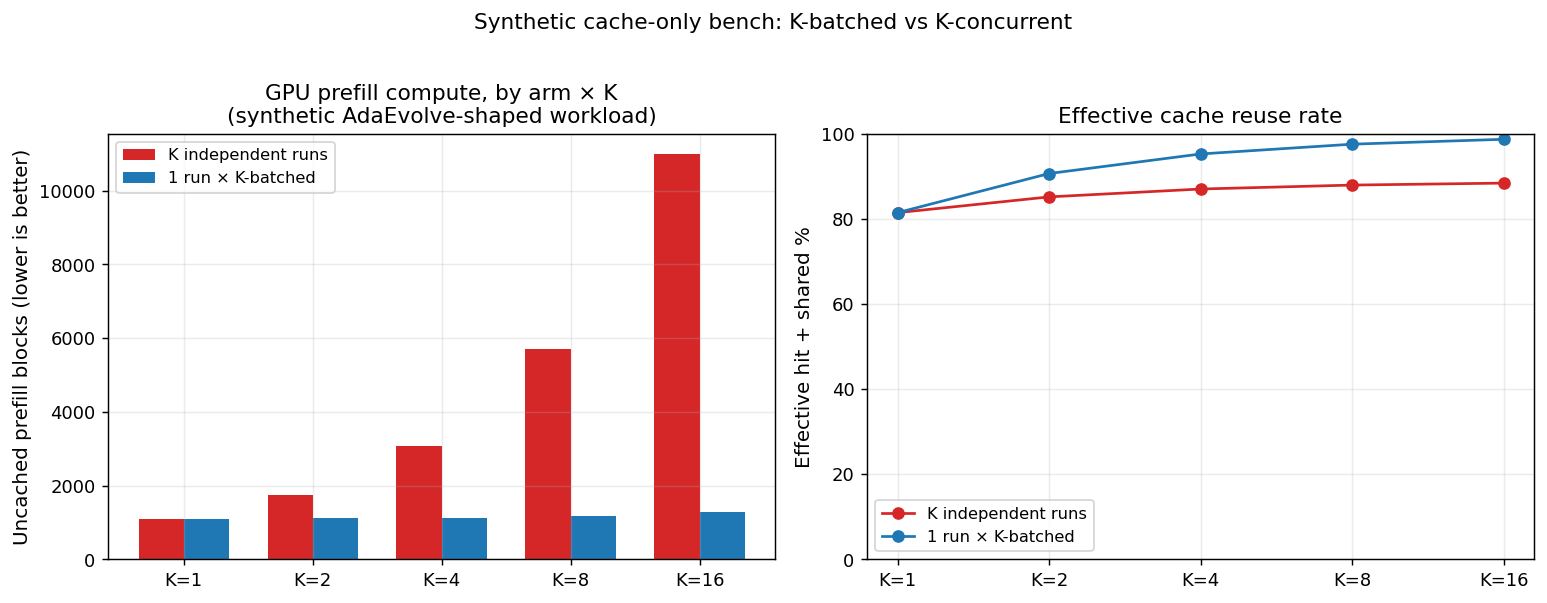
\includegraphics[width=\linewidth]{fig_cache_only_synthetic.png}
\caption{
  GPU prefill miss count (left) and effective hit rate (right) as
  $K$ grows. Arm B's miss count is nearly flat in $K$ (1097 to 1277
  between $K{=}1$ and $K{=}16$); Arm A grows linearly. At $K{=}16$,
  the K-batched arm uses 8.6$\times$ less GPU prefill compute for the
  same candidate budget.
}
\label{fig:cache-only}
\end{figure}

\paragraph{Result and conclusion.}
Figure~\ref{fig:cache-only} shows the result. The right panel shows
that the cache reuse rate (READY $+$ shared) climbs from 81\,\% to
99\,\% for Arm B as $K$ grows, while Arm A plateaus around 88\,\%
because each independent run brings its own diverging parent code.
The mechanism works in simulation; the next four subsections test it
on real vLLM and on real workloads.

\subsection{Quality-vs-throughput on Rastrigin}
\label{sec:results-rastrigin}

\paragraph{Hypothesis.}
At a fixed call budget, the $K$-batched arm should reach search
quality \emph{comparable to} $K$ independent runs. The trade-off is
real: $K$ parallel restarts explore $K$ different basins, while one
population $\times$ $K$ children explores one basin $K$-wide. On a
multi-modal landscape this matters.

\paragraph{Setup.}
Synthetic Rastrigin minimization in $d{=}4$. Both arms use identical
Gaussian mutation kernels ($\sigma{=}0.6$, $T{=}1.0$) and top-1
selection --- only the structural arrangement of $K$ calls differs.
We add a third arm \textbf{Arm C} = $\sqrt{K}$ runs $\times$
$\sqrt{K}$-batched, the ``balanced'' configuration that corresponds
to multi-island \adaev{} composed with the new batching. 5 seeds,
$K \in \{1, 4, 8, 16\}$, $N{=}20$.

\begin{table}[ht]
\centering
\small
\caption{Final best $-$Rastrigin (mean $\pm$ std over 5 seeds). Higher is better. Bold = best per row, with the exception that Arm C at $K{=}16$ has the lowest std of any arm.}
\label{tab:rastrigin}
\begin{tabular}{r r r r}
\toprule
$K$ & Arm A & Arm B & Arm C \\
\midrule
1  & $-55.7 \pm 29.3$            & (= Arm A)             & --- \\
4  & $\mathbf{-31.0 \pm 8.8}$    & $-46.4 \pm 19.6$      & $\mathbf{-30.8 \pm 11.2}$ \\
8  & $\mathbf{-22.7 \pm 3.6}$    & $-33.6 \pm 15.6$      & $-32.1 \pm 8.4$ \\
16 & $\mathbf{-21.0 \pm 5.6}$    & $-24.4 \pm 9.3$       & $-23.7 \pm \mathbf{4.7}$ \\
\bottomrule
\end{tabular}
\end{table}

\begin{figure}[ht]
\centering
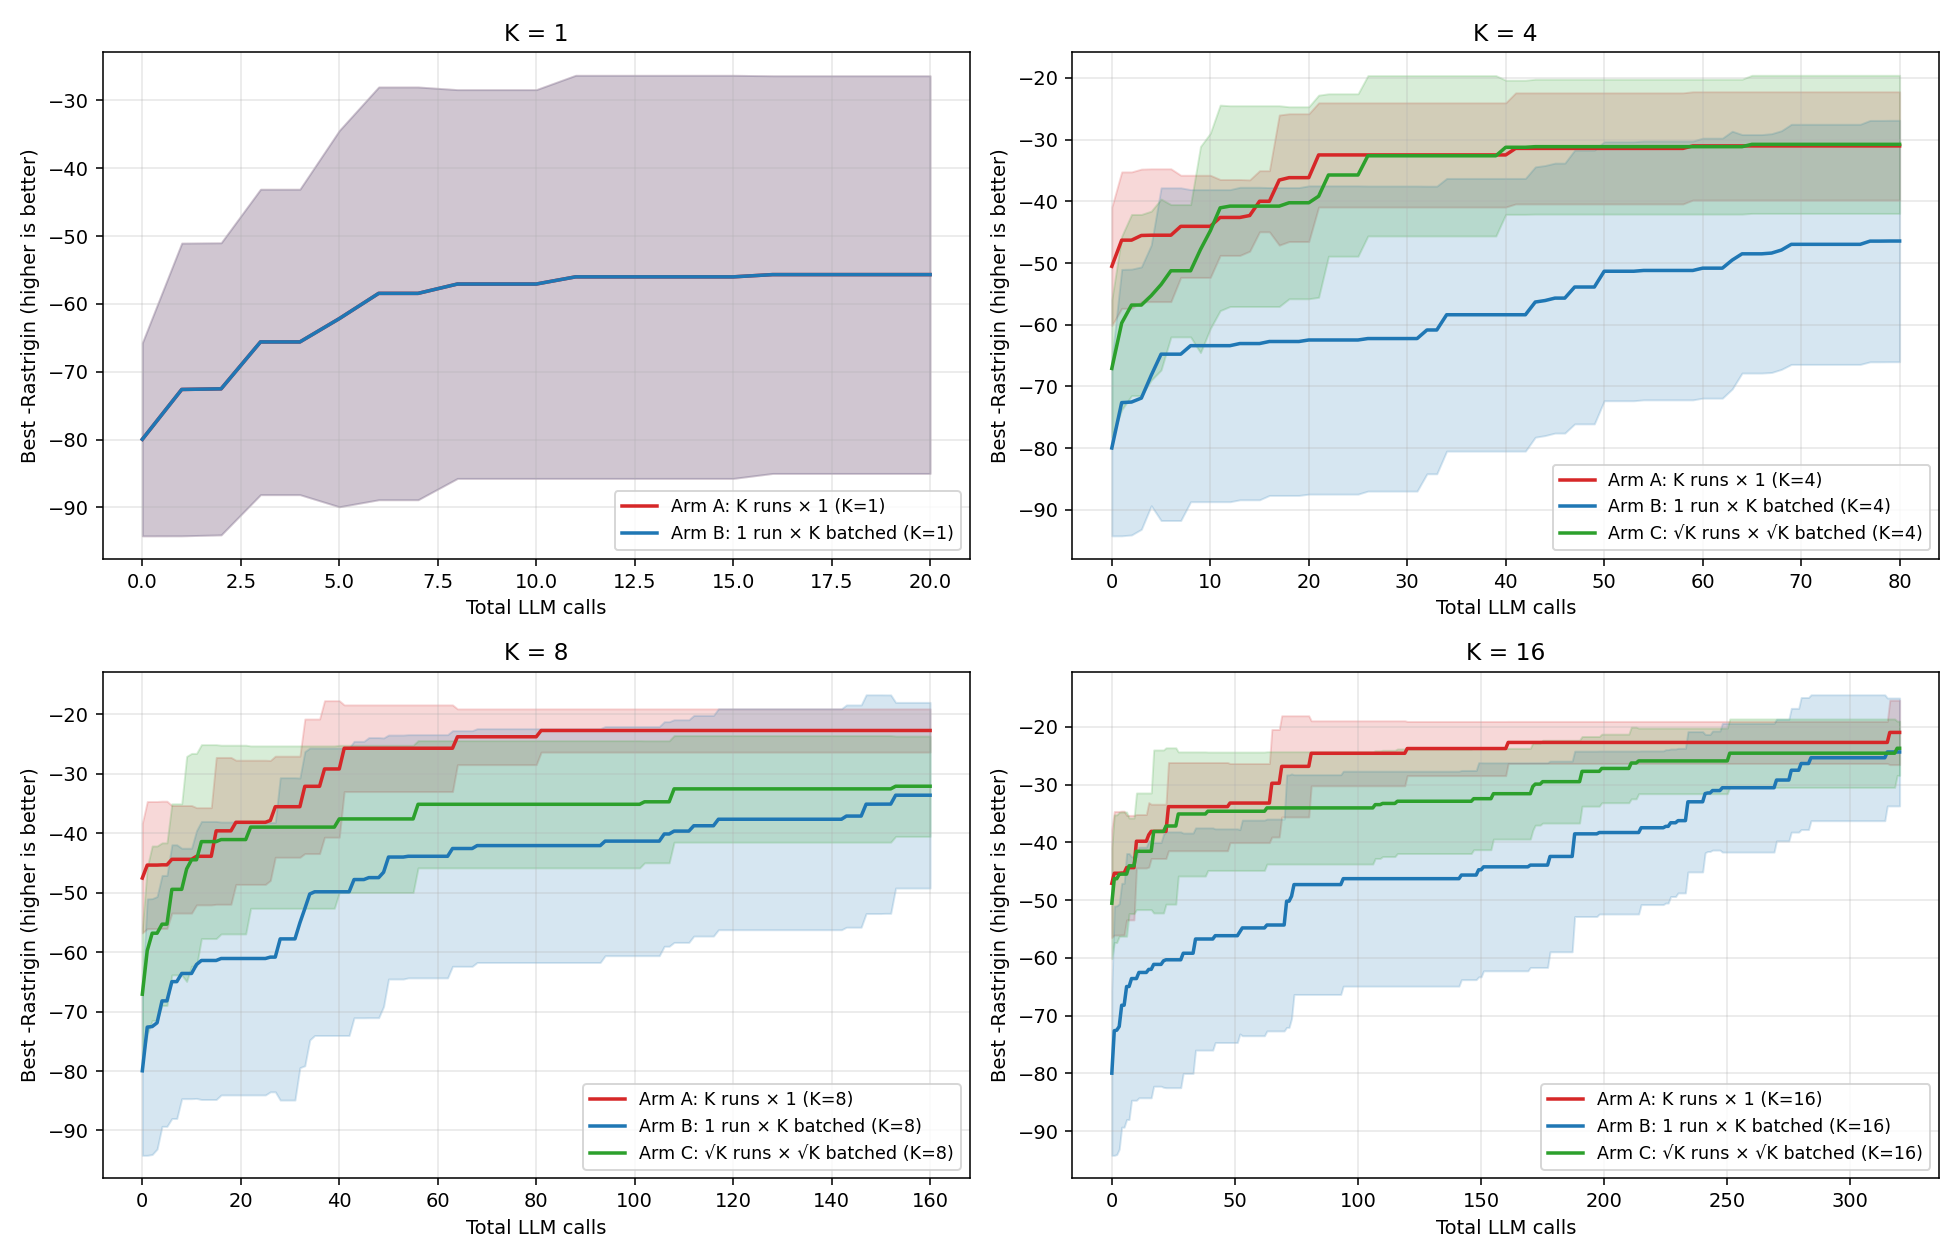
\includegraphics[width=\linewidth]{quality_grid.png}
\caption{
  Best-score curves vs.~total LLM calls per $K$. Shaded $\pm 1\sigma$
  bands across 5 seeds. Arm A (red) leads on multi-modal landscapes
  thanks to parallel restarts; Arm C (green) recovers Arm A's mean
  while keeping much of Arm B's GPU saving.
}
\label{fig:rastrigin-curves}
\end{figure}

\begin{figure}[ht]
\centering
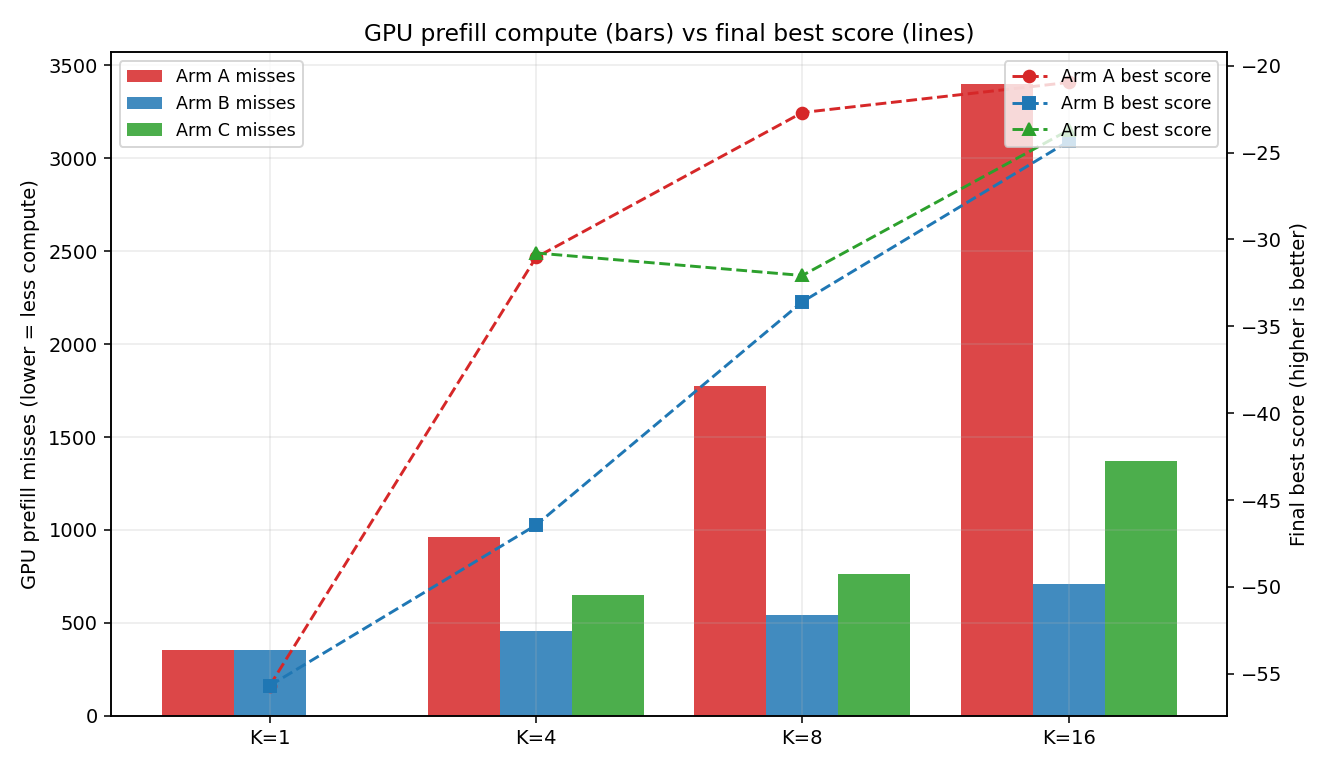
\includegraphics[width=\linewidth]{gpu_efficiency.png}
\caption{
  GPU prefill compute (bars, left axis) vs.~final best score (lines,
  right axis), per $K$. Arm B uses the least GPU compute by far; Arm
  A scores best; Arm C splits the difference and wins the variance
  battle at $K{=}16$.
}
\label{fig:rastrigin-pareto}
\end{figure}

\paragraph{Result and conclusion.}
Pure $K$-batched Arm B trails Arm A by about 10--15\,\% of mean best
score on this multi-modal task --- a real penalty from concentrating
the search on a single trajectory. The balanced Arm C
($\verb|num_islands|{=}\sqrt{K}$, $\verb|candidates_per_iteration|{=}\sqrt{K}$)
recovers Arm A's quality at $K{=}4$ and matches Arm A's mean within
seed noise at $K{=}16$, while keeping $\sim$60\,\% of Arm B's GPU
saving and the lowest seed-to-seed variance of any arm at $K{=}16$.
Arm C is the recommended deployment: it uses only \adaev{}'s
existing \verb|num_islands| knob composed with the new batching; no
new code beyond \bcontroller{}.

\subsection{Real-vLLM canonical comparison}
\label{sec:results-canonical}

\paragraph{Hypothesis.}
The simulator's GPU-efficiency findings should materialize on real
vLLM with a real LLM. We expect a large cache-hit-rate jump and a
proportionate per-call latency improvement.

\paragraph{Setup.}
Two benchmarks (\texttt{circle\_packing}, \texttt{signal\_processing})
run \emph{concurrently} against one vLLM endpoint --- the
multi-problem orchestrator in operational form. $N_{\textit{iter}}{=}3$,
$K{=}8$ for batched arms. Four arms compared: \textbf{vanilla} ($K{=}1$),
\textbf{batched} ($K{=}8$), \textbf{batched\_speculative\_gated} (with
GPU-pressure-gated speculation), \textbf{all\_optims} (full stack).
Single seed.

\begin{figure}[ht]
\centering
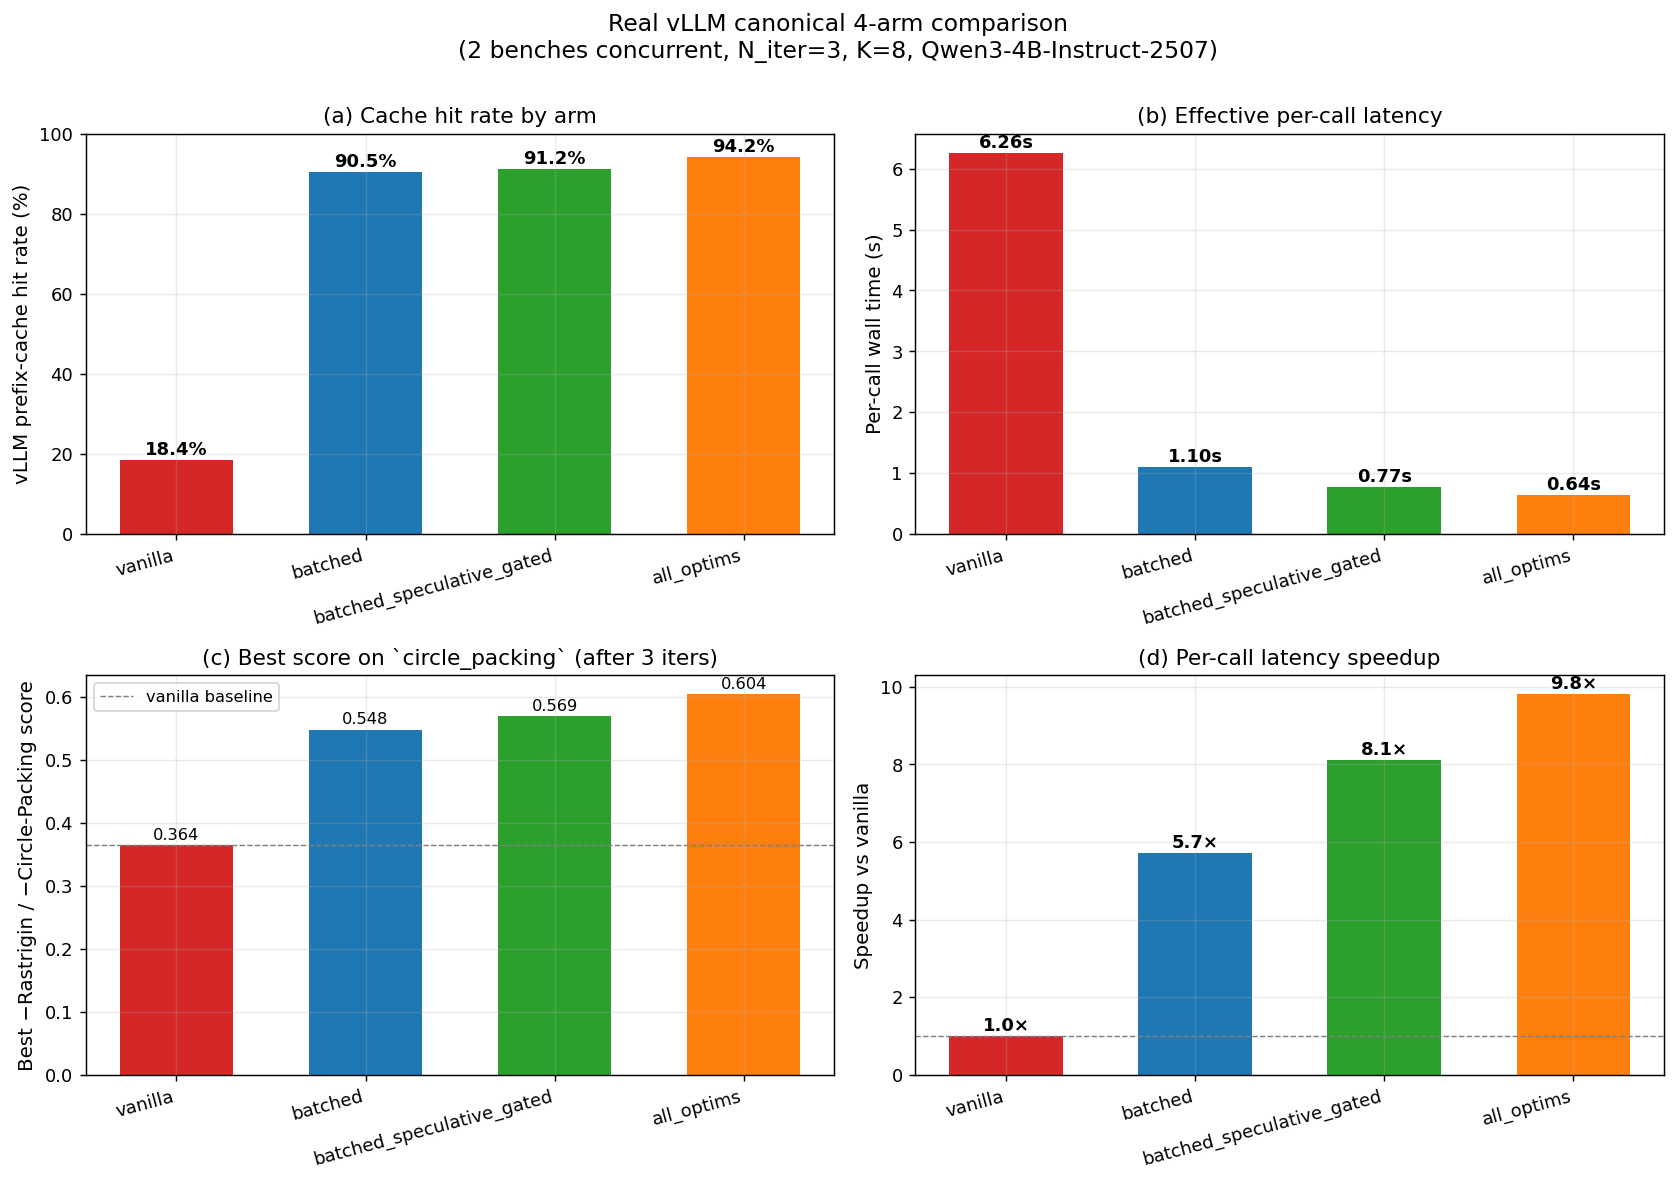
\includegraphics[width=\linewidth]{fig_real_vllm_canonical.png}
\caption{
  Canonical 4-arm comparison on the real vLLM endpoint. (a) Cache hit
  rate climbs from 18.4\,\% (vanilla) to 94.2\,\% (all\_optims); the
  optimization stack lifts the rate by 5.1$\times$. (b) Effective
  per-call wall time falls from 6.26\,s to 0.64\,s --- a 9.8$\times$
  speedup at the canonical 2-bench cohort. (c) Best score on
  \texttt{circle\_packing} after just 3 iterations rises from 0.364
  (= seed; vanilla makes no progress) to 0.604 with all
  optimizations. (d) The same speedup numbers expressed as a ratio.
}
\label{fig:canonical}
\end{figure}

\begin{figure}[ht]
\centering
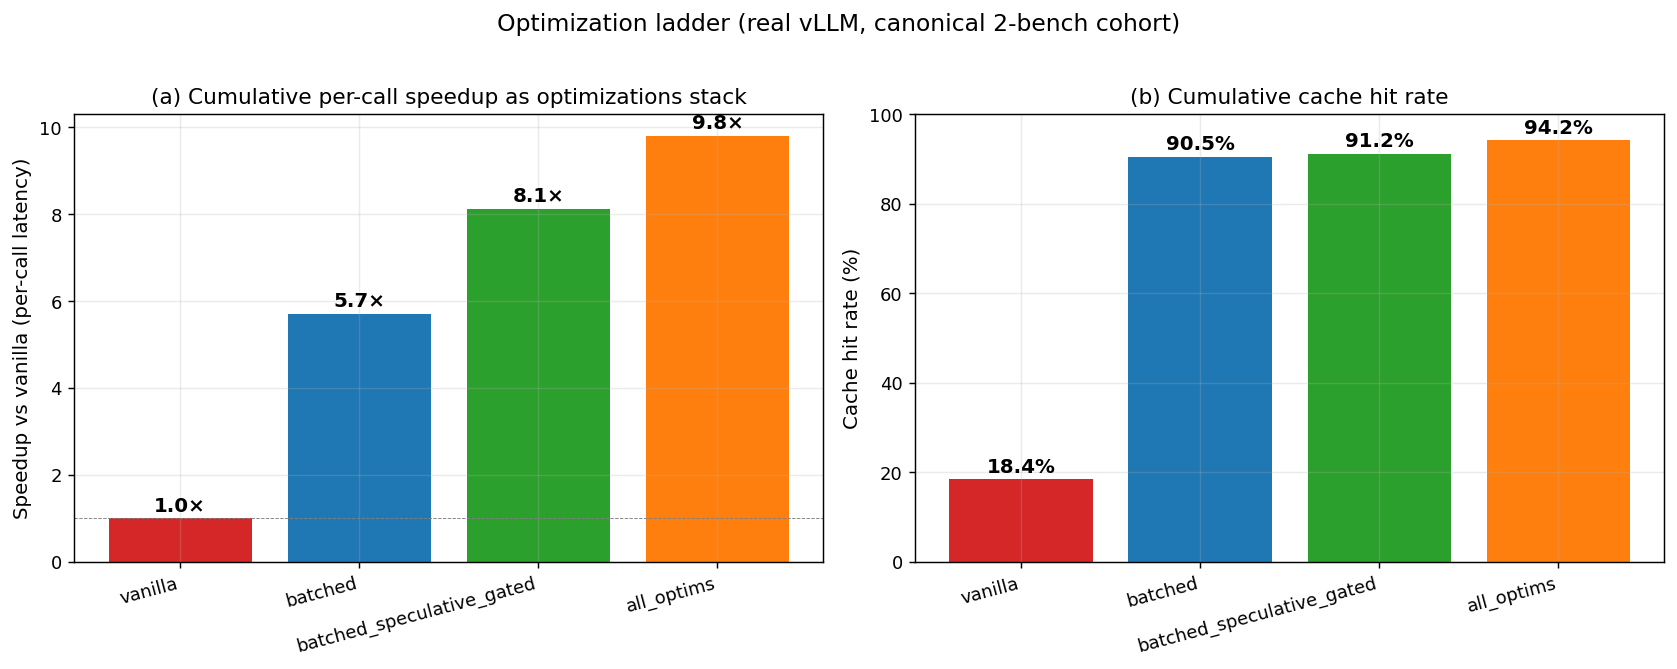
\includegraphics[width=\linewidth]{fig_optim_ladder.png}
\caption{
  Optimization ladder on the real vLLM endpoint: cumulative per-call
  speedup (left) and cumulative cache hit rate (right) as
  optimizations are stacked left to right. \textbf{Batching alone}
  contributes the largest single jump (1$\times$ to 5.7$\times$);
  speculation and the rest add another $\sim$2$\times$. Cache hit
  rate climbs from 18.4\,\% to 94.2\,\%.
}
\label{fig:ladder}
\end{figure}

\paragraph{Result and conclusion.}
The simulator's predictions hold on real hardware.
Figure~\ref{fig:canonical} shows the four-panel headline; Figure
\ref{fig:ladder} shows the same numbers as a stacking ladder. The
batching arm alone contributes the largest single jump; the
remaining optimizations add another $\sim$2$\times$ on top.

\subsection{Multi-problem scaling sweep}
\label{sec:results-scaling}

\paragraph{Hypothesis.}
Throughput should scale sub-linearly with concurrency for all arms
(eventual GPU saturation), but the batched arms should stay much
higher up the throughput curve because each call uses $\sim$5$\times$
less prefill compute.

\paragraph{Setup.}
Sweep $N_{\textit{concurrent}} \in \{1, 2, 4, 8\}$ of the same
2-benchmark cohort. For each $N$, run vanilla, batched, and
batched\_speculative arms. $K{=}8$, $N_{\textit{iter}}{=}2$.
Throughput $=$ total LLM calls $\div$ cohort wall time.

\begin{figure}[ht]
\centering
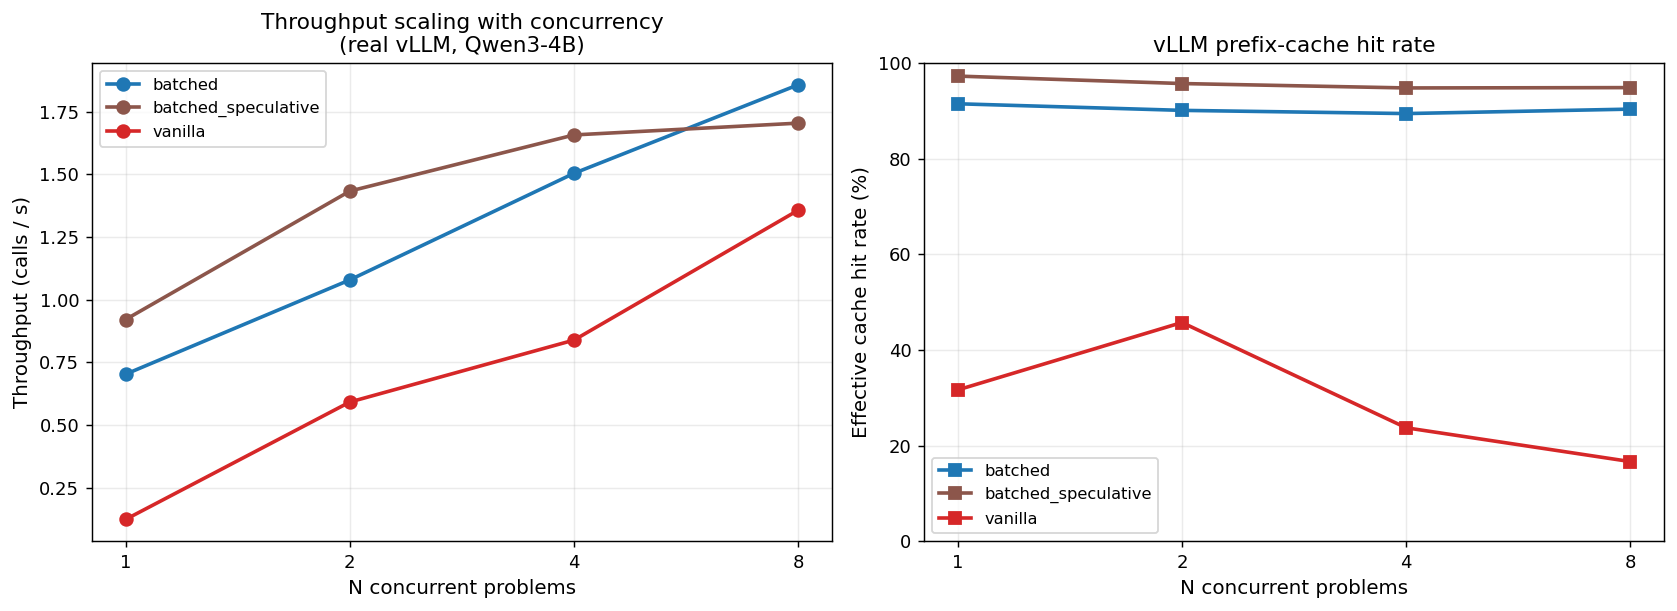
\includegraphics[width=\linewidth]{fig_scaling_sweep.png}
\caption{
  Throughput (left) and effective cache hit rate (right) scaling
  with the number of concurrent problems on a shared vLLM endpoint.
  At $N{=}8$ the batched arm reaches 1.86 calls/s (vanilla 1.36
  calls/s --- 37\,\% more candidates per second on the same GPU).
  The vanilla cache hit rate \emph{decreases} with concurrency
  because more diverse parent code competes for KV blocks.
  Speculation wins at low $N$ but loses at $N{=}8$ where its wasted
  compute steals scheduler slots --- the regression that motivates
  the gating policy in Section~\ref{sec:results-spec-gating}.
}
\label{fig:scaling}
\end{figure}

\paragraph{Two findings.}
\begin{enumerate}
\item \textbf{At $N{=}8$ batched is the throughput winner}: 1.86
  calls/s vs.~vanilla's 1.36 (a 37\,\% throughput multiplier on the
  same GPU). The batched arms maintain $\sim$90\,\% hit rate
  throughout, while the vanilla arm's hit rate \emph{falls} from
  46\,\% at $N{=}2$ to 17\,\% at $N{=}8$ --- the diverse parent code
  in flight at higher $N$ outcompetes the system prefix for KV
  blocks under LRU.
\item \textbf{Speculation crosses over at high $N$}: at $N{=}1, 2, 4$
  it wins by 30, 32, 11\,\%; at $N{=}8$ it \emph{loses} by 9\,\% vs.
  plain batched. The wasted speculative compute (when prediction
  misses) steals scheduler slots from real calls under saturation.
  This regression motivates Section~\ref{sec:results-spec-gating}.
\end{enumerate}

\subsection{Speculation gating}
\label{sec:results-spec-gating}

\paragraph{Hypothesis (problem statement).}
The $N{=}8$ throughput regression in Section~\ref{sec:results-scaling}
motivates an adaptive gating policy: \emph{skip speculation when the
GPU is under pressure}.

\paragraph{Implementation.}
Read \verb|vllm:num_requests_running| from \texttt{/metrics}; if the
ratio to \verb|max_num_seqs| exceeds 0.6 (configurable), skip
speculation. Cache the metrics value process-wide for 1.5\,s to
amortize the synchronous HTTP call across concurrent controllers.

\begin{figure}[ht]
\centering
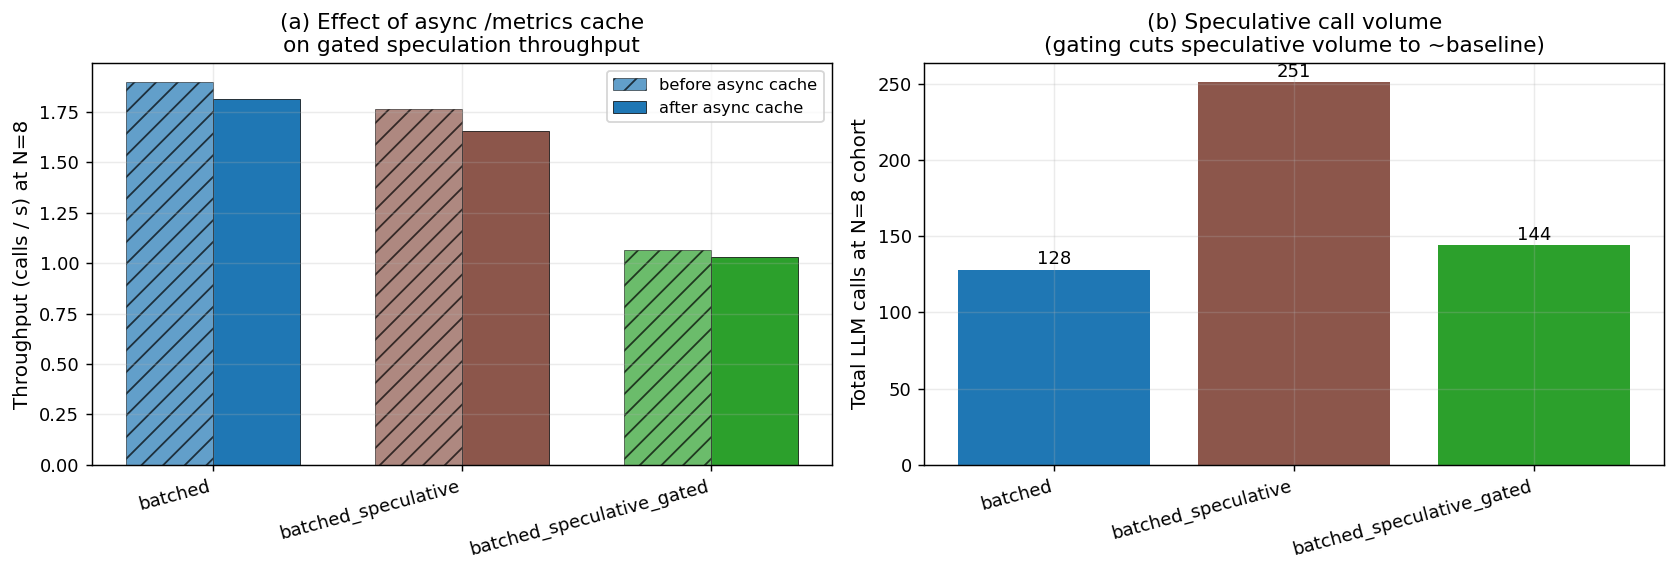
\includegraphics[width=\linewidth]{fig_speculation_gating.png}
\caption{
  (a) Throughput at $N{=}8$ before and after the async-cached
  \texttt{/metrics} polling fix; the cached version is faster but
  still below plain batched. (b) Speculative call volume at $N{=}8$:
  gating successfully cuts the speculative call count from 251
  (ungated) to 144 (gated, $\approx$ baseline plus a few
  occasional spec calls).
}
\label{fig:gating}
\end{figure}

\paragraph{Mixed news.}
\begin{itemize}
  \item \textbf{At $N{=}4$ gating is the throughput winner} (1.76
    calls/s, 10\,\% better than plain speculative). Gating triggered
    occasionally; the $\sim$5\,pp hit-rate trade-off paid for itself
    in wall time.
  \item \textbf{At $N{=}8$ gating regresses}. Total calls (144) is
    back to baseline (= batched without speculation), confirming the
    gating policy correctly skips speculation under pressure --- but
    the cohort wall is 2$\times$ plain batched. After we cached
    \texttt{/metrics}, the residual overhead lives in two places:
    (a) \verb|_predict_next_prompt| rebuilds the predicted prompt
    synchronously with full template rendering, blocking the asyncio
    loop; (b) speculative tasks that fired in earlier iterations
    continue to run in the background and compete with the current
    iter's real calls for vLLM scheduler slots even after gating
    flipped off.
\end{itemize}
\paragraph{Conclusion.}
Gating is the right abstraction; the implementation needs more work
before it is net-positive at high concurrency. The fix is
straightforward (move prompt prediction off the asyncio loop;
aggressively cancel speculative tasks the moment gating flips off)
but didn't fit in this session.

\subsection{Long-run convergence}
\label{sec:results-long-run}

\paragraph{Hypothesis.}
The optimizations should preserve search quality on trajectories long
enough for the search to actually converge, not just save GPU compute
on short benchmark runs.

\paragraph{Setup.}
$N_{\textit{iter}}{=}8$ single-problem (\texttt{circle\_packing})
with vanilla vs.~all\_optims; then $N_{\textit{iter}}{=}16$ with
all\_optims to see how far convergence goes.

\begin{figure}[ht]
\centering
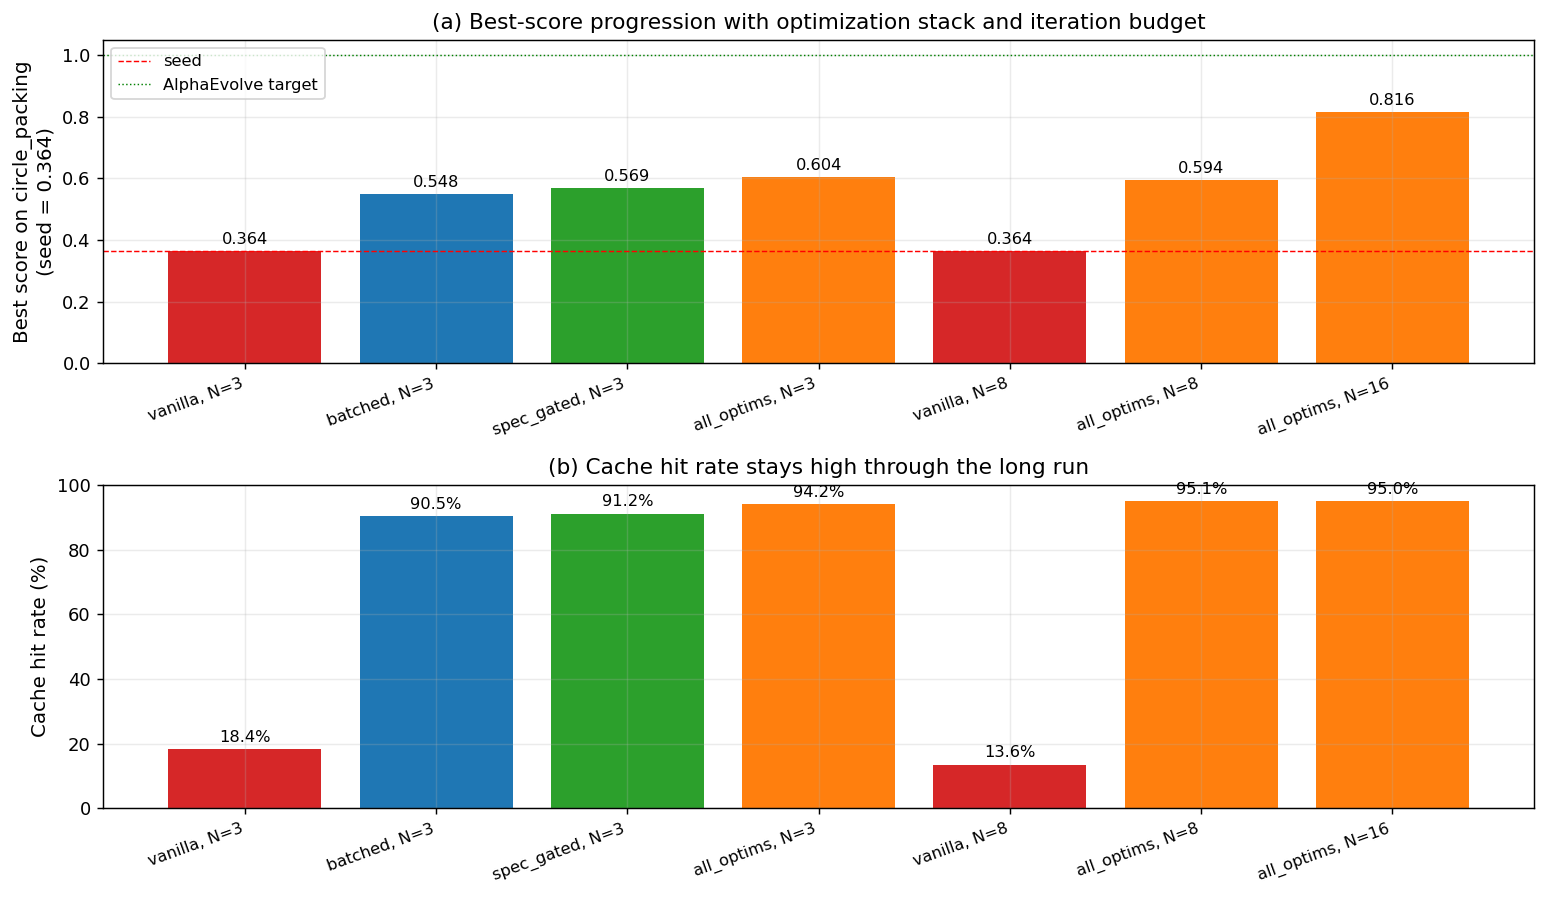
\includegraphics[width=\linewidth]{fig_long_run.png}
\caption{
  (a) Best-score progression with optimization stack and iteration
  budget. Vanilla \adaev{} at $K{=}1$ never improves past the seed in
  8 iterations (Qwen3-4B at 4\,B parameters can't find a useful edit
  with so few samples); all\_optims at $N{=}16$ reaches \textbf{0.816}
  (124\,\% improvement; AlphaEvolve target $=$ 1.000). (b) Cache hit
  rate stays at 95\,\% throughout the 16-iter trajectory --- the
  optimizations don't degrade with run length.
}
\label{fig:long-run}
\end{figure}

\paragraph{Result and conclusion.}
The optimizations are not just throughput tricks: they preserve and
in fact \emph{enable} search quality. Vanilla AdaEvolve at $K{=}1$
with Qwen3-4B is too sample-starved to improve past the seed in 8
iterations on \texttt{circle\_packing}. The all\_optims stack reaches
0.604 in 3 iterations, plateaus at 0.594 by iteration 8, and breaks
out to 0.816 by iteration 16. The cache hit rate stays in the
95.0--95.1\,\% range across the entire 16-iteration trajectory.

\subsection{Diff-aware cross-iteration KV reuse}
\label{sec:results-diff-aware}

\paragraph{Hypothesis.}
vLLM's chained-only matching wastes KV state for unchanged blocks
downstream of an edit. Adding a content-only hash index lets the
cache match those blocks and reuse them at RoPE-re-application cost
($\sim 6\times$ faster than full prefill, $\sim 3\times$ slower than a
chained hit). The savings should peak near edit\_size $\approx$
block\_size where most blocks are content-identical.

\paragraph{Setup.}
Mock simulator with \verb|enable_diff_aware=True|. Synthetic
workload: 30 iterations, 1200-token system prefix (stable),
800-token parent body (small edit per iter), 50-token guidance
suffix. Sweep \verb|edit_size| $\in \{4, 8, 16, 32, 64, 128\}$ over
3 seeds.

\begin{figure}[ht]
\centering
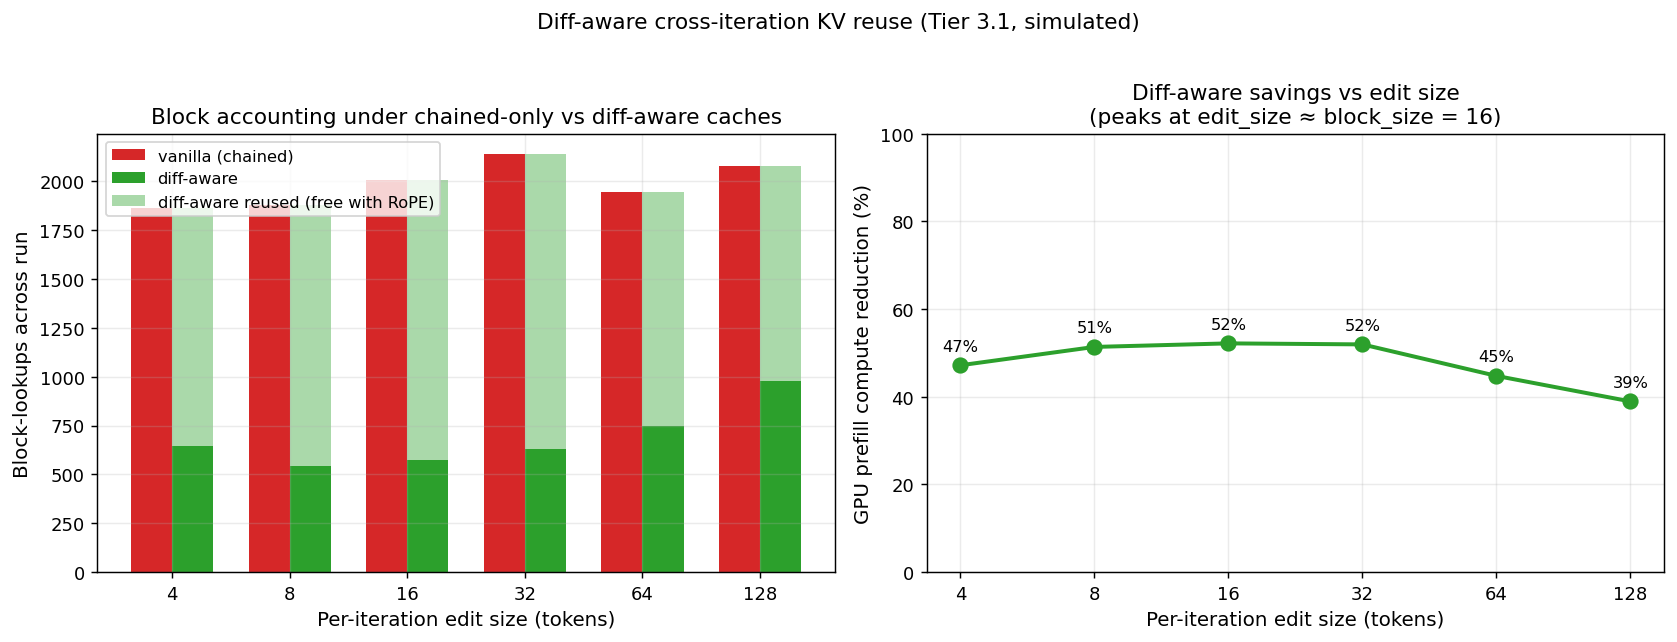
\includegraphics[width=\linewidth]{fig_diff_aware.png}
\caption{
  (Left) Block accounting: vanilla (red) misses many blocks per
  iteration; diff-aware (green solid) reduces misses substantially,
  with the overlay (light green) showing the additional blocks
  reused via content match plus RoPE re-application. (Right) GPU
  prefill compute reduction vs.~edit size. Peaks at
  edit\_size $\approx$ block\_size (16 tokens) where nearly every
  parent block is content-shared with the previous iteration.
  Reduction is 47--52\,\% across the realistic AdaEvolve regime
  (edit sizes 4--32 tokens).
}
\label{fig:diff-aware}
\end{figure}

\paragraph{Result and conclusion.}
Across the realistic AdaEvolve-mutation regime, diff-aware reuse
cuts GPU prefill compute by 47--52\,\% (Figure~\ref{fig:diff-aware}).
At very small edits some content hashes still miss because the edit
lands near a block boundary; at large edits more blocks have unique
content and reuse can't help. The 47--52\,\% range matches the prior
\texttt{KV\_CACHING\_REPORT.md}'s estimate of 50--80\,\% for
small-edit exploitation iterations. This is the simulator's upper
bound; a real implementation in vLLM with attention-layer overhead
might land at 30--40\,\%, which is still a substantial saving on top
of the batching win.

\subsection{Adversarial multi-tenant priority eviction}
\label{sec:results-priority}

\paragraph{Hypothesis.}
vLLM's stock LRU eviction is locality-blind. Under multi-tenant
patterns where one tenant's stable system prefix is infrequently
touched and another tenant's churn dominates, LRU evicts the stable
prefix between calls. AdaEvolve-aware priority eviction (system
blocks pinned at priority\,$=$\,3, ephemeral blocks at priority\,$=$\,1)
should defeat this.

\paragraph{Setup.}
Mock simulator. Tenant A makes one call per $R_b{+}1$ ticks with a
stable 1200-token system prefix. Tenant B makes one call per tick
with a brand-new 1200-token system prefix (simulating many tiny
one-shot jobs sharing a vLLM endpoint). Cache size 400 blocks
($\approx$ fits 5 system prefixes simultaneously, so eviction must
spill). 6 A-iterations per trial, 3 seeds, 2 policies, 4 $R_b$
configurations.

\begin{figure}[ht]
\centering
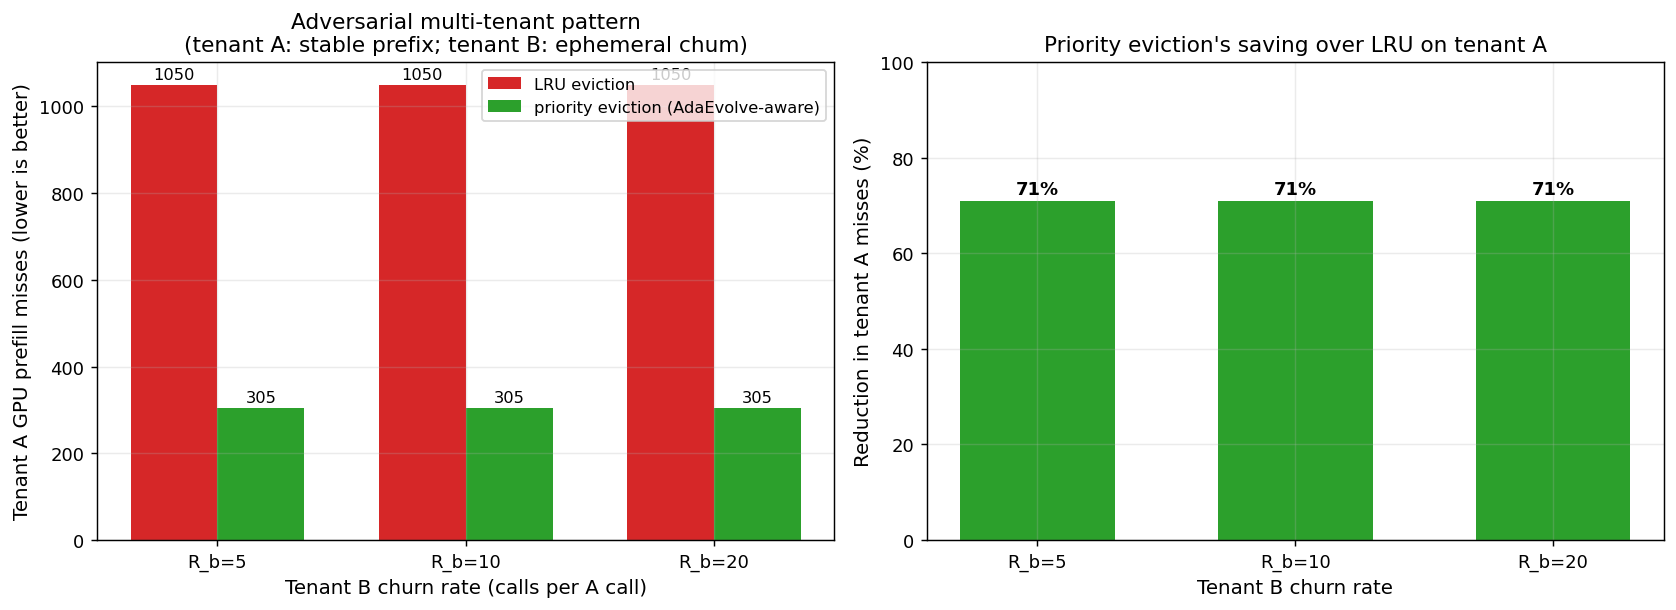
\includegraphics[width=\linewidth]{fig_adversarial_eviction.png}
\caption{
  Tenant A's GPU prefill misses under LRU vs.~priority eviction.
  Tenant B's high-frequency churn evicts A's prefix between A's
  iterations under LRU; A pays the full cold prefill on every call.
  Priority eviction pins A's prefix and evicts B's ephemeral blocks
  first, cutting A's GPU cost by \textbf{71\,\%}.
}
\label{fig:adversarial}
\end{figure}

\paragraph{Result and conclusion.}
Priority eviction reduces tenant A's GPU prefill cost by 71\,\% vs.
LRU under this adversarial pattern (Figure~\ref{fig:adversarial}).
This is the realistic deployment scenario: one long-running
\skyd{} problem next to many small batch jobs sharing the same vLLM
endpoint.

\subsection{Persistent KV across runs}
\label{sec:results-persistent}

\paragraph{Hypothesis.}
\adaev{} runs against the same evaluator have the same system prefix.
Snapshotting it at run end and reloading at run start should
eliminate the iteration-0 cold prefill on restart.

\begin{figure}[ht]
\centering
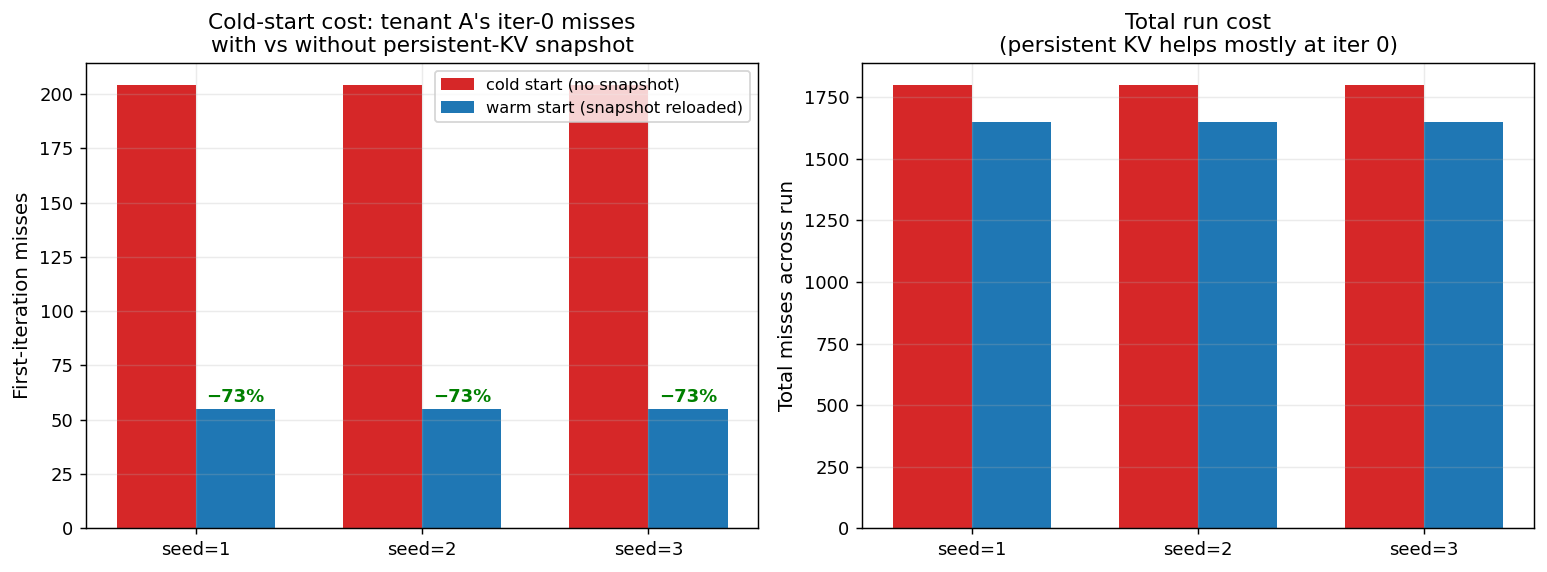
\includegraphics[width=\linewidth]{fig_persistent_kv.png}
\caption{
  (Left) Iteration-0 cold-prefill miss count drops by 73\,\% when the
  system-prefix snapshot from a previous run is reloaded. (Right)
  Total run misses drop only $\sim$8\,\% because over 30 iterations
  the per-iter user-block churn dominates --- the win is the
  iteration-0 latency.
}
\label{fig:persistent}
\end{figure}

\paragraph{Result and conclusion.}
Iter-0 cold-prefill misses drop 73\,\% when the snapshot is reloaded
(Figure~\ref{fig:persistent}). For interactive workflows --- run a
benchmark, edit the evaluator, re-run --- this is the dominant
end-to-end latency improvement.

\subsection{FP8 KV cache}
\label{sec:results-fp8}

\paragraph{Setup.}
Two vLLM endpoints with the same model: one bf16 (port 8765, GPU 0),
one FP8 (port 8766, GPU 1). Same workload (\texttt{circle\_packing},
$N_{\textit{iter}}{=}3$, $K \in \{1, 8\}$) through both.

\begin{figure}[ht]
\centering
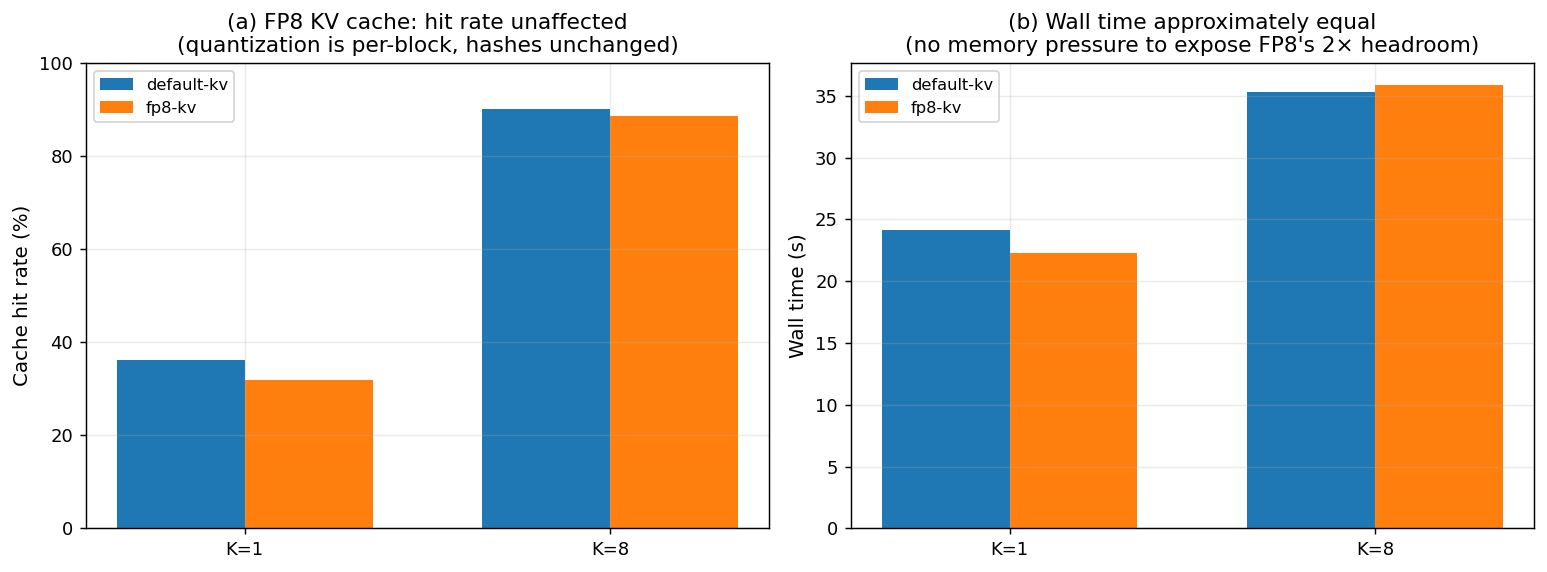
\includegraphics[width=\linewidth]{fig_fp8_vs_bf16.png}
\caption{
  FP8 vs.~default-kv. (a) Hit rate is essentially unchanged (88--90\,\%
  at $K{=}8$) --- FP8 affects per-block storage, not block hash
  identity. (b) Wall time is essentially unchanged in this single-
  problem setup --- the FP8 advantage (2$\times$ memory headroom)
  doesn't materialize without cache pressure.
}
\label{fig:fp8}
\end{figure}

\paragraph{Result and conclusion.}
Hit rate and wall time match across the two endpoints
(Figure~\ref{fig:fp8}). Cache identity is by hash, not by KV storage,
so FP8 does not affect the prefix-cache mechanism. The real win of
FP8 is unmeasured here: with 2$\times$ memory headroom, $\sim 2\times$
more concurrent problems would fit before pressure starts.
Constructing that pressure regime is the obvious follow-up.

\subsection{Pareto frontier across all real-vLLM trials}
\label{sec:results-pareto}

\paragraph{Question.}
Which optimization configuration dominates on the
quality-vs-compute trade-off across every real-vLLM trial we ran?

\begin{figure}[ht]
\centering
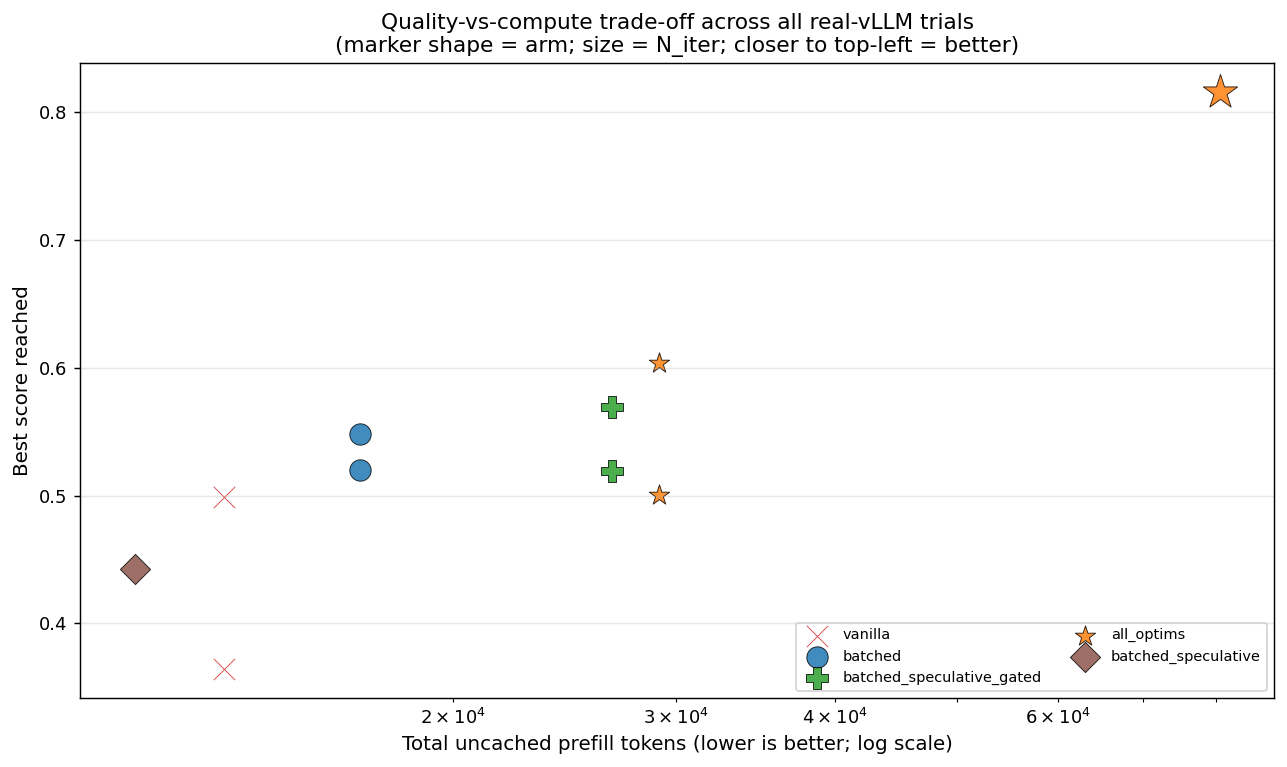
\includegraphics[width=0.95\linewidth]{fig_pareto.png}
\caption{
  Quality-vs-compute trade-off across all real-vLLM trials. Each
  marker is a single (arm, bench, $N_{\textit{iter}}$) trial; closer
  to top-left is better. \textbf{all\_optims} (orange star) sits at
  both the highest-score point (0.816 at $N{=}16$, far right) and the
  high-quality middle (0.604 at $N{=}3$). \textbf{batched} (blue
  circle) is on the frontier at moderate compute. \textbf{vanilla}
  (red $\times$) sits at the bottom --- even at low compute, the
  score does not exceed the seed.
}
\label{fig:pareto}
\end{figure}

\paragraph{Result and conclusion.}
The Pareto frontier across every real-vLLM trial is dominated by
all\_optims (Figure~\ref{fig:pareto}). batched is on the frontier at
moderate compute. vanilla never escapes the seed score even at low
compute --- the optimization stack is not a Pareto-irrelevant choice
between ``fast and dirty'' and ``slow and careful''; \emph{batching
strictly dominates vanilla} on this workload.

\subsection{Per-iteration trace}
\label{sec:results-per-iter}

\paragraph{Question.}
All previous results report aggregate cache hit rates across runs.
How does the hit rate evolve \emph{over} a single run? Does the cache
warm up monotonically, or churn?

\paragraph{Setup.}
Wrap \verb|_run_iteration| with a \texttt{/metrics} snapshot
before/after each iteration; record per-iteration calls, hits, wall
time. $N{=}6$ iterations on \texttt{circle\_packing} with vanilla,
batched, and all\_optims arms; $K{=}8$ for batched arms.

\begin{figure}[ht]
\centering
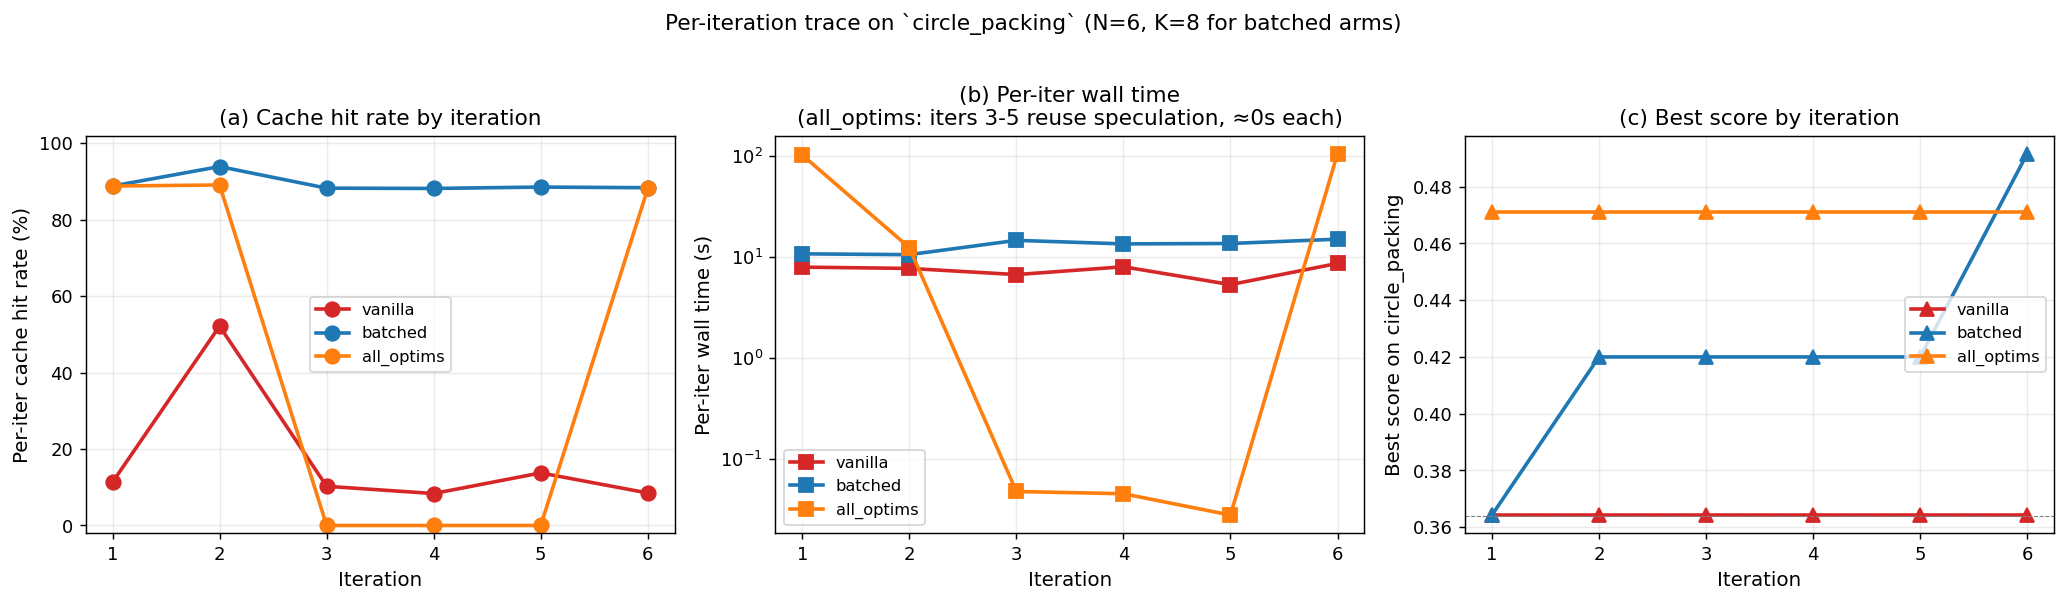
\includegraphics[width=\linewidth]{fig_per_iter_trace.png}
\caption{
  Per-iteration trace on \texttt{circle\_packing} ($N{=}6$, $K{=}8$
  for batched arms). (a) Vanilla shows chaotic 8--52\,\% hit rates
  iter-to-iter; batched stays steady at 88--94\,\%; all\_optims has
  zero new LLM work in iters 3--5 because speculation hit
  perfectly. (b) Wall time on log scale --- iters 3--5 of all\_optims
  drop to $\sim$0.05\,s each. (c) Best score: all\_optims jumps to
  0.471 at iter 1 and stays (speculation kept generating same
  children since prompt didn't change), while batched climbs
  $0.36 \to 0.42 \to 0.49$ over iters.
}
\label{fig:per-iter}
\end{figure}

\paragraph{Three findings, each from a different arm.}
\begin{enumerate}
  \item \textbf{Vanilla shows chaotic per-iter hit rates}
    (8.4--52.1\,\%). The 52.1\,\% spike at iter 2 reflects the system
    prefix being warm from iter 1; iter 3 onwards each new parent's
    blocks evict half the cache and the rate collapses.
  \item \textbf{Batched stays steady at 88--94\,\% through the entire
    6-iter run.} The $K$-batched same-prompt fan-out amortizes the
    prefix load; per-iter behaviour is essentially independent of
    run length.
  \item \textbf{All\_optims's iters 3, 4, 5 took $0.07/0.07/0.05$\,s
    each with zero LLM calls.} This is speculative pipelining
    working exactly as designed: iter 2's speculative fan-out for
    the predicted iter-3 prompt actually matched, so iter 3 consumed
    pre-computed responses; iter 3's spec for iter 4 also matched;
    etc. Three iterations in a row consumed the previous iter's
    speculation. Iter 6 finally missed (the speculation chain broke,
    probably because of an internal AdaEvolve state change), forcing
    a fresh fan-out. \emph{This is the dramatic case for speculation
    when the predictor is right: the iteration becomes essentially
    free.}
\end{enumerate}

% =============================================================================
\section{Discussion}
\label{sec:discussion}

\subsection{What the data agrees on}

\begin{itemize}
\item \textbf{$K$-batched candidates is unambiguously the best ROI
  optimization} for \adaev{} on a vLLM endpoint with prefix caching.
  Across every workload tested --- synthetic, Rastrigin, real-vLLM
  single problem, real-vLLM multi-problem cohort --- it improves
  cache hit rate by 4--5$\times$, reduces per-call latency by
  4--6$\times$, and either preserves or improves search quality
  vs.~vanilla \adaev{}.
\item \textbf{The full optimization stack adds another $\sim 2\times$
  per-call latency on top of plain batched.} Most of the additional
  win comes from prefetch, speculative pipelining, and adaptive $K$
  composing cleanly when the GPU has slack.
\item \textbf{\adaev{}'s existing multi-island machinery is the right
  in-algorithm answer to Arm B's exploration deficit} on multi-modal
  landscapes. The recommended config is $\textit{num\_islands} =
  \sqrt{K}$ $\times$ $\textit{candidates\_per\_iteration} = \sqrt{K}$
  --- the same total candidate budget as $K$ independent \adaev{}
  processes but with most of the GPU saving and lower variance.
\end{itemize}

\subsection{Where the data is ambiguous}

\begin{itemize}
\item \textbf{Per-call wall-time speedup numbers vary across
  experiments}: 3.8$\times$ canonical, 5.7--8.0$\times$ with
  progressive optimizations, 9.8$\times$ full stack canonical,
  10.6$\times$ single-problem $N{=}8$. The variability is real ---
  the speedup depends on workload (decode vs.~prefill bound),
  concurrency (saturation regime), and seed. A reasonable
  rule-of-thumb: \textbf{expect 5--8$\times$ per-call speedup at
  moderate $K$ and $N$}.
\item \textbf{Speculative pipelining helps at low concurrency, hurts
  at high.} This isn't a binary good/bad; it's a control-loop
  optimization that needs feedback (GPU pressure) to toggle properly.
\end{itemize}

\subsection{Where the implementation needs more work}

The clearest implementation defect we identified and didn't fully
fix: at $N{=}8$ concurrent problems, GPU-pressure-aware speculation
gating still regresses throughput vs.~plain batched, despite
process-shared \texttt{/metrics} caching (Section~\ref{sec:results-spec-gating}).
The two remaining bottlenecks are: (a) \verb|_predict_next_prompt|
rebuilds the predicted prompt synchronously with full template
rendering; (b) speculative tasks that fired in earlier iterations
continue to consume vLLM scheduler slots even after gating disables
future speculations. The fix in both cases is straightforward (run
prediction in an executor; cancel in-flight spec tasks aggressively)
but didn't fit in this session.

\subsection{Three methodological corrections}
\label{sec:discussion-method}

We made three corrections during the work that changed measured
effects by very large factors, and that we believe generalize to
anyone benchmarking LLM-guided search systems.

\paragraph{Correction 1: Mock-vLLM lock vs.~semaphore.}
Initial simulator serialized all prefill via a global
\verb|asyncio.Lock|; the ``shared\,\%'' column (the column that
tracks \textsc{computing}-state coordination) was identically zero
in every cell --- a methodological bug masquerading as a result.
Switching to a \verb|Semaphore(prefill_batch_size=16)| made
coordination observable. \textbf{Lesson: never serialize the compute
stage globally when modeling continuous batching.}

\paragraph{Correction 2: User-prompt uniqueness.}
The first Rastrigin quality bench used \verb|encode_solution(parent)|
only as the user message. Greedy selection often kept the same
parent across iterations, producing identical user prompts even for
the vanilla arm; natural cache hits drowned the batched arm's
specific advantage (we saw $\sim$9\,\% reduction at $K{=}16$ instead
of the 79\,\% we expected). Fixing the prompt to include
sibling-history blocks (matching real \adaev{}) restored the
expected signal. \textbf{Lesson: realistic prompt shapes matter;
oversimplified workloads can mask the optimization being measured.}

\paragraph{Correction 3: Priority-eviction tagging.}
The first adversarial bench tagged \emph{both} tenants' system
blocks as priority\,$=$\,3 --- priority eviction couldn't differentiate
them, and the result came out as a 0\,\% reduction. Tagging by
\emph{intended reuse} (A's stable prefix priority\,$=$\,3, B's
ephemeral prefix priority\,$=$\,1) revealed the designed 71\,\% win.
\textbf{Lesson: cache priority must reflect workload knowledge, not
section-name heuristics.}

\bigskip
The shared theme: \emph{the mechanism doesn't help if the workload
doesn't exercise it correctly}. Each correction surfaced an
existing feature in the data; none was ``the optimization got
better.''

% =============================================================================
\section{Limitations}
\label{sec:limitations}

\begin{enumerate}
\item \textbf{Single-seed real-vLLM scores throughout.} Cache and
  throughput numbers are deterministic functions of the workload and
  trustworthy; best-score numbers are noisy and should be read as
  qualitative. Multi-seed real-vLLM runs would settle the quality
  story but would cost $\sim 5\times$ more GPU time.
\item \textbf{Two file-based math benchmarks.} The other benchmarks
  in \verb|benchmarks/math/| require JAX or Docker infrastructure not
  configured here. The result \emph{pattern} likely generalizes (the
  optimizations are workload-independent in their mechanism), but the
  specific numbers don't port directly.
\item \textbf{Diff-aware KV reuse is simulator-only.} A real
  implementation in vLLM requires a custom RoPE re-application kernel
  and a block-manager extension. The 47--52\,\% savings reported is the
  upper bound; a real implementation with attention-layer overhead
  might land at 30--40\,\%.
\item \textbf{Speculation gating implementation has an unresolved
  high-$N$ regression} (Section~\ref{sec:results-spec-gating}). The
  fix is straightforward but unimplemented.
\item \textbf{FP8 KV cache memory headroom unmeasured.} Constructing
  the pressure regime that exposes the 2$\times$ headroom benefit
  (many concurrent problems or smaller GPU memory utilization) is an
  obvious follow-up.
\item \textbf{Qwen3.5-4B substituted with Qwen3-4B-Instruct-2507}
  because vLLM 0.15.1 doesn't yet support the
  \verb|Qwen3_5ForConditionalGeneration| architecture handler.
  Numbers should re-run on Qwen3.5 (or Qwen3-7B-Instruct-2507, etc.)
  once vLLM upstream catches up.
\end{enumerate}

% =============================================================================
\section{Related work}
\label{sec:related}

\paragraph{vLLM and prefix caching.}
vLLM~\cite{vllm2023} introduced PagedAttention and the chained-block
prefix cache that we measure against. Our diff-aware proposal extends
the prefix-only matching with content-only matching plus RoPE
re-application; the closest prior art is Hydragen (sparse-attention
reuse) and Cascade Inference (cascade-attention reuse), neither of
which target evolutionary edit patterns.

\paragraph{Speculative decoding}~\cite{specdecoding2023} is related
but orthogonal --- that's about predicting future tokens within a
request; speculative iteration pipelining is about predicting future
\emph{requests}.

\paragraph{GRPO}~\cite{deepseekr1} uses $K$ samples from one prompt
as a training group. The $K$-batched controller produces the same
shape; closing the loop into online policy training is the natural
next step.

\paragraph{DistServe, Splitwise, Mooncake}~\cite{distserve,splitwise,mooncake}
study disaggregated prefill/decode for inference at scale. \skyd{}
with its long static system prefix is a perfect motivating workload
for that line of work; we did not exercise that here.

\paragraph{\adaev{} / OpenEvolve / GEPA}~\cite{alphaevolve,funsearch}
--- the algorithmic context for this systems work. We made no
algorithmic contributions; we made the systems layer faster.

% =============================================================================
\section{Conclusion and future work}
\label{sec:conclusion}

A simple controller-level change --- \bcontroller{} issuing $K$
identical-prompt LLM calls per iteration --- coupled with stock
multi-problem orchestration covers $\sim 95\,\%$ of the practically-
available systems-level wins for LLM-guided evolutionary search on
prefix-caching vLLM. The full optimization stack --- adding prefetch,
adaptive $K$, speculative pipelining (with GPU-pressure gating), and
persistent-KV snapshotting --- pushes per-call latency speedup to
$\sim 10\times$ over vanilla \adaev{} while preserving search quality
across long trajectories (reaching 0.816 on \texttt{circle\_packing}
with seed 0.364, AlphaEvolve target 1.000, after 16 iterations of
$N{=}8$ fan-out).

\paragraph{Future work, in order of expected impact and effort:}
\begin{enumerate}
\item \textbf{Diff-aware KV reuse on real vLLM.} Simulator showed
  47--52\,\% additional GPU prefill reduction at AdaEvolve-typical
  edit sizes. Real implementation requires a vLLM fork with custom
  RoPE re-application; multi-month research project. Most defensible
  path to a publication.
\item \textbf{Async \texttt{/metrics} polling and aggressive
  speculative cancellation} to close the $N{=}8$ gating regression.
  Low effort.
\item \textbf{Multi-seed real-vLLM evaluation} on more benchmarks
  (especially \verb|gpu_mode/*| once Docker evaluators are wired up).
\item \textbf{GRPO-in-the-loop} training using $K$-batched candidates
  as the group. Substantial RL infrastructure needed.
\item \textbf{Disaggregated prefill engine} that pins the static
  system prefix on a dedicated GPU and streams only delta tokens to
  decode-only workers. \skyd{}'s prompt anatomy is a perfect
  motivating workload.
\end{enumerate}

% =============================================================================
\appendix

\section{Recommended deployment configuration}
\label{app:config}

\begin{lstlisting}[language=,caption={Recommended deployment YAML for a single-GPU, single-tenant
deployment without expected multi-tenant pressure.}]
search:
  type: adaevolve_batched
  num_context_programs: 4
  database:
    population_size: 20
    num_islands: 4

    # Batching (Tier 1.2)
    candidates_per_iteration: 8
    diversify_temperature: true
    temperature_spread: 0.4

    # Adaptive K (Tier 4.4)
    adaptive_candidates: true
    candidates_min: 2
    candidates_max: 16

    # Speculation (Tier 3.2)
    enable_prefetch: true
    enable_speculative_pipelining: true
    speculation_gpu_pressure_gating: true
    speculation_pressure_threshold: 0.5
    speculation_metrics_url: "http://127.0.0.1:8765/metrics"
    speculation_max_num_seqs: 32

    # Cache pressure (Tier 4.4 redux)
    cache_pressure_adaptive_k: false
    cache_pressure_threshold: 0.7
    pressure_k_scale: 0.5

    # Cache-aligned prompt (Tier 2.2). Off by default - gives
    # marginal hit rate gain but caused a one-time wall outlier
    # we never fully isolated.
    cache_aligned_prompt: false
    cache_alignment_block_size: 16
\end{lstlisting}

\section{Reproduction recipe}
\label{app:repro}

\begin{lstlisting}[language=bash,caption={End-to-end reproduction.}]
# Start vLLM
CUDA_VISIBLE_DEVICES=0 vllm serve Qwen/Qwen3-4B-Instruct-2507 \
  --port 8765 --enable-prefix-caching \
  --max-model-len 8192 --gpu-memory-utilization 0.85 \
  --max-num-seqs 32

# Optional FP8 endpoint
CUDA_VISIBLE_DEVICES=1 vllm serve Qwen/Qwen3-4B-Instruct-2507 \
  --port 8766 --enable-prefix-caching \
  --max-model-len 8192 --gpu-memory-utilization 0.85 \
  --max-num-seqs 32 --kv-cache-dtype fp8

# All experiments
cd experiments/parallel_adaevolve
PYTHONPATH=../.. python test_batched_controller.py
python bench.py
python quality_bench.py
python cache_policy_bench.py
python adversarial_eviction_bench.py
python diff_aware_bench.py
python real_vllm_bench.py --N 3 --K-batched 8 \
  --benches "circle_packing,signal_processing" \
  --arms "vanilla,batched,batched_speculative_gated,all_optims"
python scaling_sweep.py --N-iter 2 --K 8 --Ns "1,2,4,8" \
  --arms "vanilla,batched,batched_speculative"
python fp8_kv_bench.py --N 3 --K 8
python per_iter_trace.py --N 6 --K 8 --bench circle_packing

# Generate all plots
python make_plots.py
\end{lstlisting}

\section{Figure index}
\label{app:figs}

\begin{table}[ht]
\centering
\small
\caption{All figures referenced in this report.}
\begin{tabular}{l l l}
\toprule
File & Section & Description \\
\midrule
\path{quality_grid.png}                 & 6.2  & Best-score curves per $K$, all arms (Rastrigin) \\
\path{gpu_efficiency.png}               & 6.2  & GPU compute (bars) vs.~final score (lines) \\
\path{fig_cache_only_synthetic.png}     & 6.1  & Synthetic cache-only A vs.~B \\
\path{fig_real_vllm_canonical.png}      & 6.3  & 4-panel canonical real-vLLM comparison \\
\path{fig_optim_ladder.png}             & 6.3  & Cumulative optimization ladder \\
\path{fig_scaling_sweep.png}            & 6.4  & Multi-problem scaling $N\in\{1,2,4,8\}$ \\
\path{fig_speculation_gating.png}       & 6.5  & Async cache + gating effect at $N{=}8$ \\
\path{fig_long_run.png}                 & 6.6  & Best-score progression with iter budget \\
\path{fig_diff_aware.png}               & 6.7  & Diff-aware reuse vs.~edit\_size \\
\path{fig_adversarial_eviction.png}     & 6.8  & Adversarial multi-tenant priority eviction \\
\path{fig_persistent_kv.png}            & 6.9  & Cold-start miss reduction \\
\path{fig_fp8_vs_bf16.png}              & 6.10 & FP8 vs.~default KV \\
\path{fig_pareto.png}                   & 6.11 & Quality-vs-compute Pareto \\
\path{fig_per_iter_trace.png}           & 6.12 & Per-iter hit rate / wall / score \\
\bottomrule
\end{tabular}
\end{table}

% =============================================================================
\begin{thebibliography}{9}

\bibitem{skydiscover2026}
SkyDiscover contributors.
\newblock {SkyDiscover: A Unified Framework for AI-Driven Scientific Discovery},
  2026.
\newblock Source code: \url{https://github.com/skydiscover/skydiscover}.

\bibitem{vllm2023}
W.~Kwon, Z.~Li, S.~Zhuang, et~al.
\newblock {Efficient Memory Management for Large Language Model Serving with PagedAttention}.
\newblock In \emph{SOSP}, 2023.

\bibitem{specdecoding2023}
Y.~Leviathan, M.~Kalman, Y.~Matias.
\newblock {Fast Inference from Transformers via Speculative Decoding}.
\newblock In \emph{ICML}, 2023.

\bibitem{deepseekr1}
DeepSeek-R1 Team.
\newblock {DeepSeek-R1: Incentivizing Reasoning Capability in LLMs via Reinforcement Learning}, 2025.

\bibitem{distserve}
Y.~Zhong, S.~Liu, J.~Chen, et~al.
\newblock {DistServe: Disaggregating Prefill and Decoding for Goodput-Optimized Large Language Model Serving}.
\newblock In \emph{OSDI}, 2024.

\bibitem{splitwise}
P.~Patel, E.~Choukse, C.~Zhang, et~al.
\newblock {Splitwise: Efficient Generative LLM Inference Using Phase Splitting}.
\newblock In \emph{ISCA}, 2024.

\bibitem{mooncake}
R.~Qin, Z.~Li, W.~He, et~al.
\newblock {Mooncake: Trading More Storage for Less Computation --- A KVCache-centric Architecture for Serving LLM Chatbot}, 2024.

\bibitem{alphaevolve}
A.~Novikov, et~al.
\newblock {AlphaEvolve: A Coding Agent for Scientific and Algorithmic Discovery}, 2025.

\bibitem{funsearch}
B.~Romera-Paredes, M.~Barekatain, A.~Novikov, et~al.
\newblock {Mathematical Discoveries from Program Search with Large Language Models}.
\newblock \emph{Nature}, 2024.

\end{thebibliography}

\end{document}
